% Options for packages loaded elsewhere
\PassOptionsToPackage{unicode}{hyperref}
\PassOptionsToPackage{hyphens}{url}
%
\documentclass[
  10pt,
]{article}
\usepackage{amsmath,amssymb}
\usepackage{lmodern}
\usepackage{setspace}
\usepackage{ifxetex,ifluatex}
\ifnum 0\ifxetex 1\fi\ifluatex 1\fi=0 % if pdftex
  \usepackage[T1]{fontenc}
  \usepackage[utf8]{inputenc}
  \usepackage{textcomp} % provide euro and other symbols
\else % if luatex or xetex
  \usepackage{unicode-math}
  \defaultfontfeatures{Scale=MatchLowercase}
  \defaultfontfeatures[\rmfamily]{Ligatures=TeX,Scale=1}
\fi
% Use upquote if available, for straight quotes in verbatim environments
\IfFileExists{upquote.sty}{\usepackage{upquote}}{}
\IfFileExists{microtype.sty}{% use microtype if available
  \usepackage[]{microtype}
  \UseMicrotypeSet[protrusion]{basicmath} % disable protrusion for tt fonts
}{}
\makeatletter
\@ifundefined{KOMAClassName}{% if non-KOMA class
  \IfFileExists{parskip.sty}{%
    \usepackage{parskip}
  }{% else
    \setlength{\parindent}{0pt}
    \setlength{\parskip}{6pt plus 2pt minus 1pt}}
}{% if KOMA class
  \KOMAoptions{parskip=half}}
\makeatother
\usepackage{xcolor}
\IfFileExists{xurl.sty}{\usepackage{xurl}}{} % add URL line breaks if available
\IfFileExists{bookmark.sty}{\usepackage{bookmark}}{\usepackage{hyperref}}
\hypersetup{
  hidelinks,
  pdfcreator={LaTeX via pandoc}}
\urlstyle{same} % disable monospaced font for URLs
\usepackage[margin=1in]{geometry}
\usepackage{longtable,booktabs,array}
\usepackage{calc} % for calculating minipage widths
% Correct order of tables after \paragraph or \subparagraph
\usepackage{etoolbox}
\makeatletter
\patchcmd\longtable{\par}{\if@noskipsec\mbox{}\fi\par}{}{}
\makeatother
% Allow footnotes in longtable head/foot
\IfFileExists{footnotehyper.sty}{\usepackage{footnotehyper}}{\usepackage{footnote}}
\makesavenoteenv{longtable}
\usepackage{graphicx}
\makeatletter
\def\maxwidth{\ifdim\Gin@nat@width>\linewidth\linewidth\else\Gin@nat@width\fi}
\def\maxheight{\ifdim\Gin@nat@height>\textheight\textheight\else\Gin@nat@height\fi}
\makeatother
% Scale images if necessary, so that they will not overflow the page
% margins by default, and it is still possible to overwrite the defaults
% using explicit options in \includegraphics[width, height, ...]{}
\setkeys{Gin}{width=\maxwidth,height=\maxheight,keepaspectratio}
% Set default figure placement to htbp
\makeatletter
\def\fps@figure{htbp}
\makeatother
\setlength{\emergencystretch}{3em} % prevent overfull lines
\providecommand{\tightlist}{%
  \setlength{\itemsep}{0pt}\setlength{\parskip}{0pt}}
\setcounter{secnumdepth}{-\maxdimen} % remove section numbering
\usepackage{geometry}
\geometry{verbose,letterpaper,top=0.85in,left=2.75in,footskip=0.75in,marginparwidth=2in}

% \usepackage[breaklinks=true,pdfstartview=FitH,citecolor=blue]{hyperref}
\hypersetup{colorlinks,%
	citecolor=blue,%
	filecolor=red,%
	linkcolor=blue,%
	urlcolor=red,%
	pdfstartview=FitH}

\usepackage[T1]{fontenc}
\usepackage[utf8]{inputenc}
\usepackage{textgreek}
\usepackage[greek,english]{babel}
\usepackage{microtype}
\usepackage{amsmath}
\usepackage[osf]{libertine}
\usepackage{libertinust1math}
\usepackage{inconsolata}

\usepackage{booktabs}

\usepackage{setspace}
\doublespacing

% \setstretch{1.8999999999999999}

\usepackage[right]{lineno}

% \renewcommand{\rmdefault}{cmr}

% Additional template based on: https://www.overleaf.com/project/5dba26749d2ef50001d3a002

% clean citations
\usepackage{cite}

% hyperref makes references clicky. use \url{www.example.com} or \href{www.example.com}{description} to add a clicky url
\usepackage{nameref,hyperref}

% improves typesetting in LaTeX
\usepackage{microtype}
\DisableLigatures[f]{encoding = *, family = * }

% text layout - change as needed
\raggedright
\setlength{\parindent}{0.5cm}
\textwidth 5.25in 
\textheight 8.75in

% adjust caption style
\usepackage[aboveskip=1pt,labelfont=bf,labelsep=period,singlelinecheck=off]{caption}

% remove brackets from references
\makeatletter
\renewcommand{\@biblabel}[1]{\quad#1.}
\makeatother

% headrule, footrule and page numbers
\usepackage{lastpage,fancyhdr,graphicx}
\usepackage{epstopdf}
\pagestyle{myheadings}
\pagestyle{fancy}
\fancyhf{}
\rfoot{\thepage/\pageref{LastPage}}
\renewcommand{\footrule}{\hrule height 2pt \vspace{2mm}}
\fancyheadoffset[L]{2.25in}
\fancyfootoffset[L]{2.25in}

% use \textcolor{color}{text} for colored text (e.g. highlight to-do areas)
\usepackage{color}

% define custom colors (this one is for figure captions)
\definecolor{Gray}{gray}{.25}

% this is required to include graphics
\usepackage{graphicx}

% use if you want to put caption to the side of the figure - see example in text
\usepackage{sidecap}

% use for have text wrap around figures
\usepackage{wrapfig}
\usepackage[pscoord]{eso-pic}
\usepackage[fulladjust]{marginnote}
\reversemarginpar


% flush left while keep identation
\makeatletter
\newcommand\iraggedright{%
  \let\\\@centercr\@rightskip\@flushglue \rightskip\@rightskip
  \leftskip\z@skip}
\makeatother

% make pdf as default figure format
\DeclareGraphicsExtensions{.pdf,.png, %
    .jpg,.mps,.jpeg,.jbig2,.jb2,.JPG,.JPEG,.JBIG2,.JB2}

\usepackage{newunicodechar}
\DeclareRobustCommand{\okina}{%
  \raisebox{\dimexpr\fontcharht\font`A-\height}{%
    \scalebox{0.8}{`}%
  }%
}
\newunicodechar{ʻ}{\okina}
\ifluatex
  \usepackage{selnolig}  % disable illegal ligatures
\fi
\newlength{\cslhangindent}
\setlength{\cslhangindent}{1.5em}
\newlength{\csllabelwidth}
\setlength{\csllabelwidth}{3em}
\newenvironment{CSLReferences}[2] % #1 hanging-ident, #2 entry spacing
 {% don't indent paragraphs
  \setlength{\parindent}{0pt}
  % turn on hanging indent if param 1 is 1
  \ifodd #1 \everypar{\setlength{\hangindent}{\cslhangindent}}\ignorespaces\fi
  % set entry spacing
  \ifnum #2 > 0
  \setlength{\parskip}{#2\baselineskip}
  \fi
 }%
 {}
\usepackage{calc}
\newcommand{\CSLBlock}[1]{#1\hfill\break}
\newcommand{\CSLLeftMargin}[1]{\parbox[t]{\csllabelwidth}{#1}}
\newcommand{\CSLRightInline}[1]{\parbox[t]{\linewidth - \csllabelwidth}{#1}\break}
\newcommand{\CSLIndent}[1]{\hspace{\cslhangindent}#1}

\author{}
\date{\vspace{-2.5em}}

\begin{document}

% align only at left, not at right.
\iraggedright

\setstretch{1.5}
\begin{flushleft}
{\Large
\textbf\newline{Developmental integration cannot explain major features of stomatal anatomical evolution in seed plants}
}
\newline
\\
Christopher D. Muir\textsuperscript{1,*},
Miquel \`{A}ngel Conesa\textsuperscript{2},
Jeroni Galm\'{e}s\textsuperscript{2},
Varsha S. Pathare\textsuperscript{3},
Patricia Rivera\textsuperscript{4},
Rosana López Rodríguez\textsuperscript{5},
Teresa Terrazas\textsuperscript{4},
Dongliang Xiong\textsuperscript{6}
\\
\bigskip
\bf{1} School of Life Sciences, University of Hawaiʻi at M\=anoa, Honolulu, HI 96822, USA \\
\bf{2} Research Group on Plant Biology under Mediterranean Conditions, Departament de Biologia, Universitat de les Illes Balears, Ctra. Valldemossa km 7.5, E-07122, Palma, Spain \\
\bf{3} School of Biological Sciences, Washington State University, Pullman, WA 99164-4236, USA \\
\bf{4} Departamento de Botánica, Instituto de Biología, Universidad Nacional Autónoma de México, Apartado Postal 70‑367, 04510 Mexico City, Mexico \\
\bf{5} Departamento de Sistemas y Recursos Naturales, Universidad Politécnica de Madrid, 28040 Madrid, Spain \\
\bf{6} National Key Laboratory of Crop Genetic Improvement, MOA Key Laboratory of Crop Ecophysiology and Farming System in the Middle Reaches of the Yangtze River, College of Plant Science and Technology, Huazhong Agricultural University, Wuhan, Hubei 430070, China\\
\bigskip
* cdmuir@hawaii.edu

\end{flushleft}

\hypertarget{abstract}{%
\section{Abstract}\label{abstract}}

\begin{itemize}
\tightlist
\item
  Developmental integration can cause traits to covary over macroevolutionary time and in some cases prevent populations from reaching their adaptive optima. Developmental integration between stomatal size and density may contribute to two major features of stomatal anatomical evolution: inverse size-density scaling and bimodal stomatal ratio. If these patterns result from developmental integration, we predicted that in amphistomatous leaves 1) stomatal size and density should covary similarly on both abaxial and adaxial surfaces and 2) stomatal traits (size and density) on each surface should covary isometrically.
\item
  We synthesized data on stomatal density and length from amphistomatous leaves of 711 terrestrial seed plant taxa mostly from the literature. We estimated the covariance in divergence between stomatal traits from 327 phylogenetically independent contrasts using a robust Bayesian model.
\item
  Adaxial stomatal density, but not length, is evolutionarily labile and not strongly integrated with stomatal length or abaxial stomatal density. Hence, developmental integration alone cannot explain inverse size-density scaling nor bimodal stomatal ratio.
\item
  Quasi-independent evolution of stomatal anatomical traits facilitates largely unfettered access to fitness optima. If stomatal anatomical traits are near their current fitness optimum, this implies that limits on trait (co)variance result from selective rather than developmental constraints. However, we cannot rule out that developmental integration is important in some lineages. Future research should identify the mechanistic basis of (dis)integration in stomatal development.
\end{itemize}

\textbf{Keywords:} Adaptation, amphistomy, developmental integration, leaf, phylogenetic comparative methods, stomata

\linenumbers

\hypertarget{introduction}{%
\section{Introduction}\label{introduction}}

The ability for traits to evolve independently of one another is a necessary prerequisite for adaptation to complex environments (\protect\hyperlink{ref-lewontin_adaptation_1978}{Lewontin 1978}). If traits can evolve independently and there is sufficient genetic variation, then selection should move populations toward their multivariate phenotypic optimum. Adaptive evolution may be constrained if traits cannot evolve independently because they are developmentally integrated. Developmentally integrated traits have a ``disposition for covariation'' (\protect\hyperlink{ref-armbruster_integrated_2014}{Armbruster et al. 2014}), meaning that evolutionary divergence between lineages in one character will be tightly associated with divergence in another character. Allometry is a classic example of developmental integration that may constrain phenotypic evolution (reviewed in \protect\hyperlink{ref-pelabon_evolution_2014}{Pélabon et al.} (\protect\hyperlink{ref-pelabon_evolution_2014}{2014})). Strong allometric covariation between traits within populations can constrain macroevolutionary divergence for long periods of time depending on the strength and direction of selection (\protect\hyperlink{ref-lande_quantitative_1979}{Lande 1979}). However, developmental integration does not necessarily hamper adaptation, and can even accelerate adaptive evolution when trait covariation is aligned with the direction of selection (\protect\hyperlink{ref-hansen_is_2003}{Hansen 2003}). For example, fusion of floral parts increases their developmental integration which may increase the rate and precision of multivariate adaptation to specialist pollinators (Berg's rule) (\protect\hyperlink{ref-berg_general_1959}{Berg 1959}, \protect\hyperlink{ref-berg_ecological_1960}{1960}; \protect\hyperlink{ref-conner_raissa_2014}{Conner and Lande 2014}; \protect\hyperlink{ref-armbruster_covariance_1999}{Armbruster et al. 1999}). In this study we are interested in quantifying the strength of developmental integration in stomatal anatomy and whether developmental integration might hamper or accelerate adaptive evolution.

Stomata are microscopic pores on the leaf or other photosynthetic surfaces of most land plants formed by a pair of guard cells. Here we limit our focus to stomatal traits on leaves within terrestrial seed plants, primarily angiosperms. The density, size, and patterning of stomata on a leaf set the maximum stomatal conductance to CO\(_2\) diffusing into a leaf and the amount of water that transpires from it (\protect\hyperlink{ref-sack_hydrology_2003}{Sack et al. 2003}; \protect\hyperlink{ref-franks_effect_2001}{Franks and Farquhar 2001}; \protect\hyperlink{ref-galmes_leaf_2013}{Galmés et al. 2013}). Plants typically operate below their anatomical maximum by dynamically regulating stomatal aperture. Even though operational stomatal conductance determines the realized photosynthetic rate and water-use efficiency, anatomical parameters are useful in that they set the range of stomatal function (\protect\hyperlink{ref-de_boer_optimal_2016}{Boer et al. 2016}) and are correlated with actual stomatal function under natural conditions (\protect\hyperlink{ref-murray_consistent_2020}{Murray et al. 2020}).

Two salient features of stomatal anatomy have been recognized for decades but we do not yet understand the evolutionary forces that generate and maintain them. We denote these two features as ``inverse size-density scaling'' and ``bimodal stomatal ratio'' (Fig. \ref{fig:concepts}). Inverse size-density scaling refers to the negative interspecific correlation between the size of the stomatal apparatus and the density of stomata (\protect\hyperlink{ref-weiss_untersuchungen_1865}{Weiss 1865}; \protect\hyperlink{ref-franks_maximum_2009}{Franks and Beerling 2009}; \protect\hyperlink{ref-de_boer_optimal_2016}{Boer et al. 2016}; \protect\hyperlink{ref-sack_developmental_2016}{Sack and Buckley 2016}; \protect\hyperlink{ref-liu_scaling_2021}{Liu et al. 2021}). Across species, leaves with smaller stomata tend to pack them more densely, but there is significant variation about this general trend (Fig. \ref{fig:concepts}a). Bimodal stomatal ratio refers to the observation that the ratio of stomatal density on the adaxial (upper) surface to the density on the abaxial (lower) has distinct modes (Fig. \ref{fig:concepts}b). Stomata are most often found only on the lower leaf surface (hypostomy), but occur on both surfaces (amphistomy) in some species (\protect\hyperlink{ref-metcalfe_anatomy_1950}{Metcalfe and Chalk 1950}; \protect\hyperlink{ref-parkhurst_adaptive_1978}{Parkhurst 1978}; \protect\hyperlink{ref-mott_adaptive_1982}{Mott, Gibson, and O'Leary 1982}), especially herbaceous plants from open, high light habitats (\protect\hyperlink{ref-salisbury_i_1928}{Salisbury 1928}; \protect\hyperlink{ref-mott_adaptive_1982}{Mott, Gibson, and O'Leary 1982}; \protect\hyperlink{ref-gibson_structure-function_1996}{Gibson 1996}; \protect\hyperlink{ref-smith_associations_1998}{W. K. Smith, Bell, and Shepherd 1998}; \protect\hyperlink{ref-jordan_using_2014}{Jordan, Carpenter, and Brodribb 2014}; \protect\hyperlink{ref-muir_making_2015}{Muir 2015}, \protect\hyperlink{ref-muir_light_2018}{2018}; \protect\hyperlink{ref-bucher_stomatal_2017}{Bucher et al. 2017}). \protect\hyperlink{ref-muir_making_2015}{Muir} (\protect\hyperlink{ref-muir_making_2015}{2015}) described bimodal stomatal ratio formally but the pattern is apparent in earlier comparative studies of the British flora (\emph{cf.} \protect\hyperlink{ref-peat_comparative_1994}{Peat and Fitter} (\protect\hyperlink{ref-peat_comparative_1994}{1994}) Fig 1). For both features, we limit our focus in this study to interspecific variation in mean trait values and do not seek to understand intraspecifc variation.

\begin{figure}[ht]
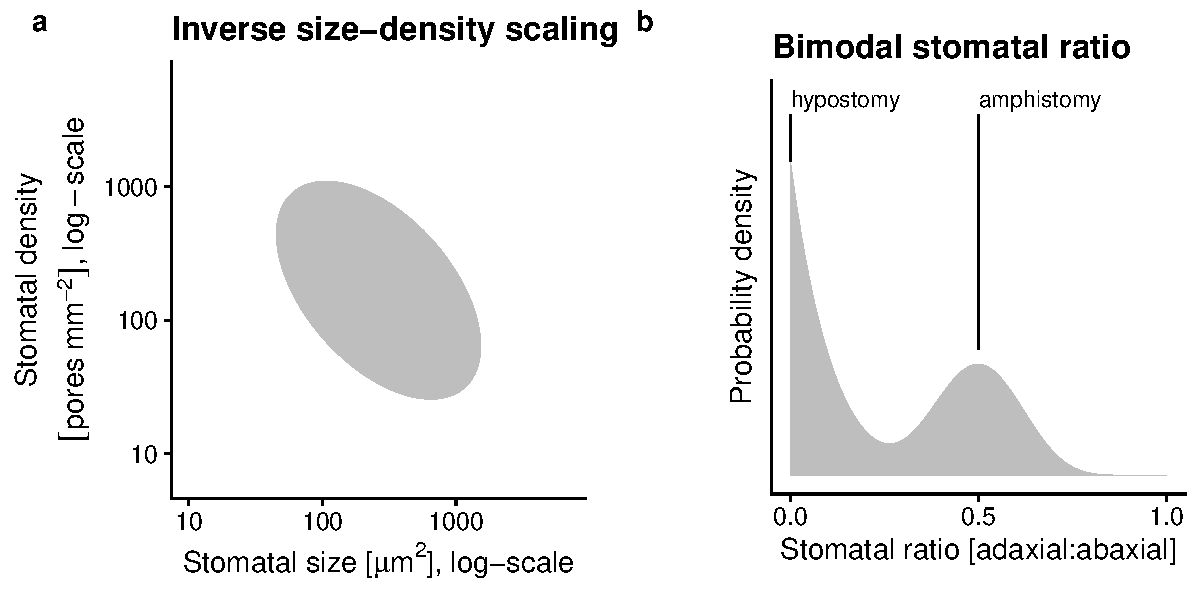
\includegraphics[width=\textwidth]{../figures/concepts.pdf}
\caption{Two salient features of stomatal anatomy in land plants are the (a) inverse relationship between stomatal size and density and (b) the bimodal distribution of stomatal ratio. At broad phylogenetic scales, leaves with smaller stomata ($x$-axis, log-scale) tend to have greater stomatal density  ($x$-axis, log-scale), but there is a lot of variation about the overall trend indicated by the grey ellipse. Hypostomatous leaves (stomatal ratio = 0) are more common than amphistomatoues leaves, but within amphistomatous leaves, the density of stomata on each surface tends to be similar (stomatal ratio $\approx$ 0.5), which we refer to as bimodal stomatal ratio.}
\label{fig:concepts}
\end{figure}

Given the significance of stomata for plant function and global vegetation modeling, we would like to understand whether these major anatomical features are shaped primarily by adaptive or nonadaptive evolutionary forces. We briefly review adaptive hypotheses for both inverse size-density scaling and bimodal stomatal ratio. Then we discuss how developmental integration might contribute to these features, in addition to or in lieu of adaptive evolution. Stomatal size and density determine the maximum stomatal conductance to CO\(_2\) and water vapor but also take up space on the epidermis, which could be costly for both construction and maintenance. Natural selection should favor leaves that have enough stomata of sufficient size to supply CO\(_2\) for photosynthesis. Hence leaves with few, small stomata and high photosynthetic rates do not exist because they would not supply enough CO\(_2\). Conversely, excess stomata or extra large stomata beyond the optimum may result in stomatal interference (\protect\hyperlink{ref-zeiger_stomatal_1987}{Zeiger, Farquhar, and Cowan 1987}), incur metabolic costs (\protect\hyperlink{ref-deans_optimization_2020}{Deans et al. 2020}), and/or risk hydraulic failure (\protect\hyperlink{ref-henry_stomatal_2019}{Henry et al. 2019}). The distribution of stomata and density may therefore represent the combinations that ensure enough, but not too much, stomatal conductance. \protect\hyperlink{ref-franks_maximum_2009}{Franks and Beerling} (\protect\hyperlink{ref-franks_maximum_2009}{2009}) further hypothesized that the evolution of small stomata in angiosperms enabled increased stomatal conductance while minimizing the epidermal area allocated to stomata.

Developmental integration between stomatal size and density, mediated by meristematic cell volume, could also explain inverse size-density scaling. If the size of both guard cells and the size of pavement cells between stomata are determined by initial meristematic cell volume, then changes in cell volume early in leaf development would cause both increased stomatal size and lower density (\protect\hyperlink{ref-brodribb_unified_2013}{Brodribb, Jordan, and Carpenter 2013}). This type of developmental integration would not hinder adaptive evolution when the main axes of selection were aligned with the developmental correlation. For example, if higher maximum stomatal conductance were achieved primarily by increasing stomatal density and decreasing stomatal size as proposed by \protect\hyperlink{ref-franks_maximum_2009}{Franks and Beerling} (\protect\hyperlink{ref-franks_maximum_2009}{2009}), then developmental integration might accelerate the response to selection compared to a case where stomatal size and density are completely independent.

The adaptive significance of variation in stomatal ratio is unknown, but we have some clues based on the distribution of hypo- and amphistomatous leaves. The functional significance of amphistomy is that it adds a second parallel pathway from the substomatal cavities through the leaf internal airspace to sites of carboxylation in the mesophyll (\protect\hyperlink{ref-parkhurst_adaptive_1978}{Parkhurst 1978}; \protect\hyperlink{ref-gutschick_photosynthesis_1984}{Gutschick 1984}). Thus amphistomatous leaves have lower resistance to diffusion through the airspace which increases the photosynthetic rate (\protect\hyperlink{ref-parkhurst_intercellular_1990}{Parkhurst and Mott 1990}). Despite this amphistomy advantage, most leaves are hypostomatous, suggesting that the benefits of amphistomy in terms of increased photosynthesis usually do not outweigh the costs of stomata on the upper surface. Amphistomy should increase photosynthesis under saturating-light conditions where CO\(_2\) supply limits photosynthesis. This may explain why amphistomatous leaves are most common in high light habitats (\protect\hyperlink{ref-salisbury_i_1928}{Salisbury 1928}; \protect\hyperlink{ref-mott_adaptive_1982}{Mott, Gibson, and O'Leary 1982}; \protect\hyperlink{ref-gibson_structure-function_1996}{Gibson 1996}; \protect\hyperlink{ref-smith_associations_1998}{W. K. Smith, Bell, and Shepherd 1998}; \protect\hyperlink{ref-jordan_using_2014}{Jordan, Carpenter, and Brodribb 2014}; \protect\hyperlink{ref-muir_making_2015}{Muir 2015}; \protect\hyperlink{ref-bucher_stomatal_2017}{Bucher et al. 2017}), especially in herbs (\protect\hyperlink{ref-muir_light_2018}{Muir 2018}). However, the light environment alone cannot explain why hypostomatous leaves predominate in shade plants (\protect\hyperlink{ref-muir_is_2019}{Muir 2019}), suggesting that we need to understand the costs of upper stomata better. Upper stomata increase the susceptibility to rust pathogens in \emph{Populus} (\protect\hyperlink{ref-mckown_association_2014}{McKown et al. 2014}, \protect\hyperlink{ref-mckown_role_2019}{2019}; \protect\hyperlink{ref-fetter_growthdefense_2021}{Fetter, Nelson, and Keller 2021}). Amphistomy may also cause the palisade mesophyll to dry out under strong vapor pressure deficits (\protect\hyperlink{ref-buckley_how_2015}{Buckley et al. 2015}). Other hypotheses about the adaptive significance of stomatal ratio are discussed in \protect\hyperlink{ref-muir_making_2015}{Muir} (\protect\hyperlink{ref-muir_making_2015}{2015}) and \protect\hyperlink{ref-drake_two_2019}{Drake et al.} (\protect\hyperlink{ref-drake_two_2019}{2019}).

A striking feature of the interspecific variation in stomatal ratio is that trait values are not uniformly distributed, but strongly bimodal. \protect\hyperlink{ref-muir_making_2015}{Muir} (\protect\hyperlink{ref-muir_making_2015}{2015}) derived general conditions in which bimodality arises because adaptive optima are restricted to separate regimes, but this model has not been tested. An alternative hypothesis is that stomatal traits on the ab- and adaxial surfaces are developmentally integrated because stomatal development is regulated the same way on each surface. In hypostomatous leaves, stomatal development is turned off in the adaxial surface. In amphistomatous leaves, stomatal development proceeds on both surfaces, but evolutionary changes in stomatal development affect traits on both surfaces because they are tethered by a shared developmental program. This model of developmental integration would lead to a bimodal trait distribution because leaves would either be hypostomatous (stomatal ratio equal to 0) or have similar densities on each surface (stomatal ratio approximately 0.5). To our knowledge, this hypothesis has not been put forward in the literature but came about during discussion with one of us (Muir, personal communication with EJ Edwards).

We reasoned that the developmental hypotheses for inverse size-density scaling and bimodal stomatal ratio could be tested using amphistomatous leaves. Since both leaf surfaces are formed from the same genome and meristematic cells, if developmental integration is strong we would expect similar patterns of trait covariation in the abaxial and adaxial surface (see below for specific predictions). Conversely, if traits covary differently on each surface it would indicate that stomatal anatomical traits can be developmentally disintegrated. Analogously, variation in the genetic correlation and interspecific divergence of sexually dimorphic traits in dioecious species demonstrate that integration is not fixed and can be modified by selection (\protect\hyperlink{ref-barrett_sexual_2013}{Barrett and Hough 2013}). Below we reiterate the hypotheses and specific predictions for amphistomatous leaves:

\noindent {\bf{Inverse size-density scaling}}

\begin{itemize}
\item
  \emph{Hypothesis}: Meristematic cell volume mediates developmental integration between stomatal size and density
\item
  \emph{Prediction}: Amphistomatous leaves will exhibit identical size-density scaling on each surface
\end{itemize}

\noindent {\bf{Bimodal stomatal ratio}}

\begin{itemize}
\item
  \emph{Hypothesis}: Stomatal traits on both leaf surfaces are developmentally integrated because they follow the same developmental program
\item
  \emph{Prediction}: Evolutionary divergence in stomatal traits on one surface will be isometric with divergence in stomatal traits on the other surface
\end{itemize}

We tested these predictions in a phylogenetic comparative framework by compiling stomatal anatomy data from the literature for a broad range of seed plants.

\hypertarget{materials-and-methods}{%
\section{Materials and Methods}\label{materials-and-methods}}

Unless otherwise mentioned, we performed all data wrangling and statistical analyses in \emph{R} version 4.1.0 (\protect\hyperlink{ref-r_core_team_r:_2021}{R Core Team 2021}). Source code is publically available on GitHub (\url{https://github.com/cdmuir/stomata-independence}) and will be archived on Zenodo upon publication.

\hypertarget{data-synthesis}{%
\subsection{Data synthesis}\label{data-synthesis}}

We searched the literature for studies that measured stomatal density and stomatal size, either guard cell length or stomatal pore length, for both abaxial and adaxial leaf surfaces. In other words, we did not include studies unless they reported separate density and size values for each surface. We did not record leaf angle because it is typically not reported, but we presume that for the vast majority of taxa that the abaxial is the lower surface and the adaxial is the upper surface. This is reversed in resupinate leaves, but to the best of our knowledge, our synthesis did not include resupinate leaves. We refer to guard cell length as stomatal length and converted stomatal pore length to stomatal length assuming guard cell length is twice pore length (\protect\hyperlink{ref-sack_developmental_2016}{Sack and Buckley 2016}). Table \ref{tab:traits} lists focal traits and symbols.

\begin{longtable}[]{@{}
  >{\centering\arraybackslash}p{(\columnwidth - 4\tabcolsep) * \real{0.20}}
  >{\centering\arraybackslash}p{(\columnwidth - 4\tabcolsep) * \real{0.52}}
  >{\centering\arraybackslash}p{(\columnwidth - 4\tabcolsep) * \real{0.28}}@{}}
\caption{\label{tab:traits}Stomatal anatomical traits with mathemtical symbol, variable string used in source code, and scientific units.}\tabularnewline
\toprule
Symbol & Variable string & Units \\
\midrule
\endfirsthead
\toprule
Symbol & Variable string & Units \\
\midrule
\endhead
\(D_\mathrm{ab}\) & \(\mathtt{abaxial\_stomatal\_density\_mm2}\) & \(\text{pores mm}^{-2}\) \\
\(D_\mathrm{ad}\) & \(\mathtt{adaxial\_stomatal\_density\_mm2}\) & \(\text{pores mm}^{-2}\) \\
\(L_\mathrm{ab}\) & \(\mathtt{abaxial\_stomatal\_length\_um}\) & \(\mu\)m \\
\(L_\mathrm{ad}\) & \(\mathtt{adaxial\_stomatal\_length\_um}\) & \(\mu\)m \\
\bottomrule
\end{longtable}

Data on stomatal anatomy are spread over a disparate literature and we have not attempted an exhaustive synthesis of amphistomatous leaf stomatal anatomy. We began our search by reviewing papers that cited key studies of amphistomy (\protect\hyperlink{ref-parkhurst_adaptive_1978}{Parkhurst 1978}; \protect\hyperlink{ref-mott_adaptive_1982}{Mott, Gibson, and O'Leary 1982}; \protect\hyperlink{ref-muir_making_2015}{Muir 2015}). We supplemented these by searching Clarivate \emph{Web of Science} for ``guard cell length'' because most studies that report guard cell length also report stomatal density, whereas the reverse is not true. We identified additional studies by reviewing the literature cited of papers we found and through haphazard discovery. The final data set contained 5104 observations of stomatal density and length from 1242 taxa and 38 primary studies (Table \ref{tab:sources}). However, many of these data were excluded if taxonomic name and phylogenetic placement could not be resolved (see below). Finally, we included some previously unpublished data. Stomatal size data were collected on grass species previously described (\protect\hyperlink{ref-pathare_increased_2020}{Pathare, Koteyeva, and Cousins 2020}). We also included a previously unpublished set of 14 amphistomatous wild tomato species (\emph{Solanum} sect. \emph{Lycopersicum} and sect. \emph{Lycopersicoides}) grown in pots under outdoor summer Mediterranean conditions previously described (\protect\hyperlink{ref-muir_unpublished_2021}{Muir, Galmés, and Conesa 2021}). We took ab- and adaxial epidermal imprints using clear nail polish of the mid-portion of the lamina away from major veins on the terminal leaflet of the youngest, fully expanded leaf from 1-5 replicates per taxon. With a brightfield light microscope, we counted stomata in three fields of view and divided by area to obtain density and measured the average guard cell length to estimate stomatal size. The data set is publicly available as an \emph{R} package \textbf{ropenstomata} (\url{https://github.com/cdmuir/ropenstomata}). It will be deposited on Dryad and archived on Zenodo upon publication.

\hypertarget{phylogeny}{%
\subsection{Phylogeny}\label{phylogeny}}

We resolved taxonomic names using the R package \textbf{taxize} version 0.9.99 (\protect\hyperlink{ref-chamberlain_taxize_2013}{Chamberlain and Szöcs 2013}). We queried taxonomic names supplied by the original study authors on 2021-08-26 from the following sources: GRIN Taxonomy for Plants (\protect\hyperlink{ref-united_states_department_of_agriculture_agricultural_research_service_germplasm_2020}{United States Department of Agriculture, Agricultural Research Service 2020}), Open Tree of Life Reference Taxonomy (\protect\hyperlink{ref-rees_automated_2017}{Rees and Cranston 2017}), The International Plant Names Index (\protect\hyperlink{ref-the_royal_botanic_gardens_international_2020}{The Royal Botanic Gardens et al. 2020}), Tropicos - Missouri Botanical Garden (\protect\hyperlink{ref-missouri_botanical_garden_tropicos_2020}{Missouri Botanical Garden 2020}). We retained the maximum scoring matched name with taxize score \(\ge 0.75\) (a score of 1 is a perfect match). In 5 ambiguous cases we manually curated names. Taxonomic name resolution reduced the data set from 1224 to 1183 taxa. Most taxa are different species, but some recognized subspecies and varieties are also included. All algorithms and choices are documented in the associated source code.

We used the R packages \textbf{taxonlookup} version 1.1.5 (\protect\hyperlink{ref-pennell_simple_2016}{Pennell, FitzJohn, and Cornwell 2016}) and \textbf{V.phylomaker} version 0.1.0 (\protect\hyperlink{ref-jin_vphylomaker_2019}{Jin and Qian 2019}) to maximize overlap between our data set and the GBOTB.extended mega-tree of seed plants (\protect\hyperlink{ref-smith_constructing_2018}{S. A. Smith and Brown 2018} ; \protect\hyperlink{ref-zanne_three_2014}{Zanne et al. 2014}). We further resolved large (\(\ge4\) taxa) polytomies in 30 clades with sufficient sequence data using \textbf{PyPHLAWD} version 1.0 (\protect\hyperlink{ref-smith_pyphlawd_2019}{S. A. Smith and Walker 2019}) in Python 3.8.2 (Python Software Foundation, \url{https://www.python.org/}). We used sequence data from the most recent GenBank Plant and Fungal sequences database division (\protect\hyperlink{ref-ouellette_database_1997}{Ouellette and Boguski 1997}). We inferred subtree phylogenies using RAxML version 8.2.12 (\protect\hyperlink{ref-stamatakis_raxml_2014}{Stamatakis 2014}) and conducated molecular dating using the \texttt{chronos()} function in the R package \textbf{ape} version 5.5 (\protect\hyperlink{ref-paradis_ape_2019}{Paradis and Schliep 2019}) to obtain ultrametric trees. We grafted resolved, ultrametric subtrees onto the mega-tree at the polytomy nodes and rescaled to keep the mega-tree ultrametric. In some cases, resolving polytomies was not possible because there was little or no overlap between taxa in the data set and taxa with sequence data available for \textbf{PyPHLAWD}. In these cases, we randomly selected two taxa as a phylogenetially independent pair and dropped the rest. Remaining polytomies of three taxa were resolved randomly using the \texttt{multi2di()} function in \textbf{ape}. The final data set for which we had both trait and phylogenetic information contained 711 taxa (Notes S1). Seven taxa are gymnosperms; the vast majority are angiosperms.

\hypertarget{phylogenetically-independent-contrasts}{%
\subsection{Phylogenetically independent contrasts}\label{phylogenetically-independent-contrasts}}

We extracted 327 phylogenetically independent taxon pairs (Table \ref{tab:pair_div}). A fully resolved, bifurcating four-taxon phylogeny can have two basic topologies: \(\tt{((A,B),(C,D))}\) or \(\tt{((A,B),C),D))}\). Taxon pairs include all comparisons of \(\tt{A}\) with \(\tt{B}\) and \(\tt{C}\) with \(\tt{D}\) in each four-taxon clade. We extracted pairs using the \texttt{extract\_sisters()} function in R package \textbf{diverge} version 2.0.1 (\protect\hyperlink{ref-anderson_diverge_2021}{Anderson and Weir 2021}) and custom scripts (see source code). Taxon pairs are the most closely related pairs in our data set, but not usually the most closely related species in nature. For each pair we calculated phylogenetically independent contrasts (\protect\hyperlink{ref-felsenstein_phylogenies_1985}{Felsenstein 1985}) as the difference in the log\(_{10}\)-transformed trait value. Contrasts are denoted as \(\Delta \text{log(trait)}\). We log-transformed traits for normality because like many morphological and anatomical traits they are strongly right-skewed. Log-transformation also helps compare density and length, which are measured on different scales, because log-transformed values quantify proportional rather than absolute divergence. We only used pairs of terminal taxa rather than the entire tree for two reasons. First, even in whole-tree methods, approximately half of the data comes from divergence at the tips, so we do not lose much statistical power. Second, using a taxon-pair method obviates making strong assumptions about multivariate trait evolution process homogeneity throughout seed plant evolution. Homogeneity is biologically unlikely and it is difficult to fit more complex models reliably with only data from extant taxa.

\hypertarget{parameter-estimation}{%
\subsection{Parameter estimation}\label{parameter-estimation}}

Both hypotheses make predictions about trait covariance matrices or parameters derived from them (see next subsections). We estimated the \(4 \times 4\) covariance matrix of phylogenetically independent contrasts between log-transformed values of \(\Delta \text{log}(D_\mathrm{ab})\), \(\Delta \text{log}D_\mathrm{ad})\), \(\Delta \text{log}(L_\mathrm{ab})\), and \(\Delta \text{log}(L_\mathrm{ad})\) using a distributional multiresponse robust Bayesian approach. We denote variances as \(\text{Var}[\Delta \text{log(trait)}]\) and covariances as \(\text{Cov}[\Delta \text{log(trait}_1),\Delta \text{log(trait}_2)]\). The statistical model also accounts for differences in mean trait values between surfaces.

We used a multivariate \(t\)-distribution rather than a Normal distribution because estimates using the former are more robust to exceptional trait values. Exceptional trait values are common in biology and can distort estimates of central tendency and variance. The \(t\)-distribution is more robust because it has fatter tails (more kurtosis) than the Normal distribution. The \(\nu\) parameter of the \(t\)-distribution describes how fat the tails are. As \(\nu \to \infty\), the \(t\)-distribution converges to the Normal distribution. We estimated \(\nu\) from the data, meaning that if exceptional values are absent from the data, the model will be nearly equivalent to standard Normal regression.

We also estimated whether the variance in trait divergence increases with time. Under many trait evolution models (e.g.~Brownian motion), interspecific variance increases through time. To account for this, we included time since taxon-pair divergence as an explanatory variable affecting the trait covariance matrix, but not the trait mean.

We fit the model in Stan 2.27 (\protect\hyperlink{ref-stan_development_team_stan_2021}{Stan Development Team 2021}) using the R packages \textbf{brms} version 2.16.0 (\protect\hyperlink{ref-burkner_brms_2017}{Bürkner 2017}, \protect\hyperlink{ref-burkner_advanced_2018}{2018}) with a \textbf{cmdstanr} version 0.4.0 backend (\protect\hyperlink{ref-gabry_cmdstanr_2021}{Gabry and Češnovar 2021}). It ran on 2 parallel chains for 1000 warm-up iterations and 1000 sampling iterations. All parameters converged (\(\hat{R} \approx 1\)) and the effective sample size from the posterior exceeded 1000 (\protect\hyperlink{ref-vehtari_rank-normalization_2021}{Vehtari et al. 2021}). We used the posterior median for point estimates and calculated uncertainty with the 95\% highest posterior density (HPD) interval from the posterior distribution.

\hypertarget{is-size-density-scaling-the-same-on-both-leaf-surfaces}{%
\subsection{Is size-density scaling the same on both leaf surfaces?}\label{is-size-density-scaling-the-same-on-both-leaf-surfaces}}

We tested the first hypothesis by estimating the covariance between divergence in stomatal length and stomatal density on each leaf surface. If size and density are developmentally integrated, we predict the covariance matrices will not be significantly different. Specifically, the 95\% HPD intervals of the difference in covariance parameters should not include 0 if:

\begin{gather}\label{eq:prediction1}
\text{Var}[\Delta \text{log}(D_\text{ab})] \ne \text{Var}[\Delta \text{log}(D_\text{ad})] \\
\text{Var}[\Delta \text{log}(L_\text{ab})] \ne \text{Var}[\Delta \text{log}(L_\text{ad})] \\
\text{Cov}[\Delta \text{log}(L_\text{ab}), \Delta \text{log}(D_\text{ab})] \ne \text{Cov}[\Delta \text{log}(L_\text{ad}), \Delta \text{log}(D_\text{ad})]
\end{gather}

\hypertarget{do-abaxial-and-adaxial-stomatal-traits-evolve-isometrically}{%
\subsection{Do abaxial and adaxial stomatal traits evolve isometrically?}\label{do-abaxial-and-adaxial-stomatal-traits-evolve-isometrically}}

If stomatal traits on each surface are developmentally integrated then divergence in the trait on one surface should result in a 1:1 (isometric) change in the trait on the other surface. Furthermore, there should be relatively little variation away from a 1:1 relationship. Conversely, if traits can evolve independently then the change in the trait on one surface should be uncorrelated with changes on the other. We tested for isometry by estimating the standardized major axis (SMA) slope of change in the abaxial trait against change in the adaxial trait for both stomatal length and stomatal density. If change on each surface is isometric, then the HPD intervals for the slope should include 1. We used the coefficient of determination, \(r^2\), to quantify the strength of integration, where a value of 1 is complete integration and a value of 0 is complete disintegration.

\hypertarget{results}{%
\section{Results}\label{results}}

\hypertarget{adaxial-stomatal-density-is-more-variable-but-size-density-covariance-is-similar-on-both-surfaces}{%
\subsection{Adaxial stomatal density is more variable, but size-density covariance is similar on both surfaces}\label{adaxial-stomatal-density-is-more-variable-but-size-density-covariance-is-similar-on-both-surfaces}}

Stomatal length negatively covaries with stomatal density similarly on both surfaces, but on the adaxial surface there are many more taxa that have low stomatal density and small size compared to the abaxial surface (Fig. \ref{fig:h1_raw}). In principle, this pattern could arise either because size-density covariance differs or the variance in adaxial stomatal density increases faster than that for abaxial stomatal density. Also note that the interspecific variance increases with time since divergence for all traits (Table \ref{tab:modeloutput}), but the covariance matrix structure did not change qualitatively over time (results not shown). For consistency, we therefore report estimates conditional on time since divergence set to 0. Across pairs, we estimate that the covariance between size and density is similar. The median estimate is \(\text{Cov}[\Delta \text{log}(L_\text{ad}), \Delta \text{log}(D_\text{ad})] - \text{Cov}[\Delta \text{log}(L_\text{ab}), \Delta \text{log}(D_\text{ab})] = 2.66 \times 10^{-3}\), but 0 is within the range of uncertainty (95\% HPD interval \([-6.72 \times 10^{-4},6.79 \times 10^{-3}]\)). However the variance in adaxial stomatal density is significantly greater than the abaxial stomatal density {[}Fig. \ref{fig:h1}{]}). We estimate \(\text{Var}[\Delta \text{log}(D_\text{ad})]\) is \(2.64 \times 10^{-2}\) (95\% HPD interval \([8.40 \times 10^{-3},5.13 \times 10^{-2}]\)) greater than \(\text{Var}[\Delta \text{log}(D_\text{ab})]\). The variance in stomatal length was similar for both surfaces, with an estimate of \(-8.08 \times 10^{-5}\) (95\% HPD interval \([-1.38 \times 10^{-3},1.23 \times 10^{-3}]\)).

\begin{figure}[ht]
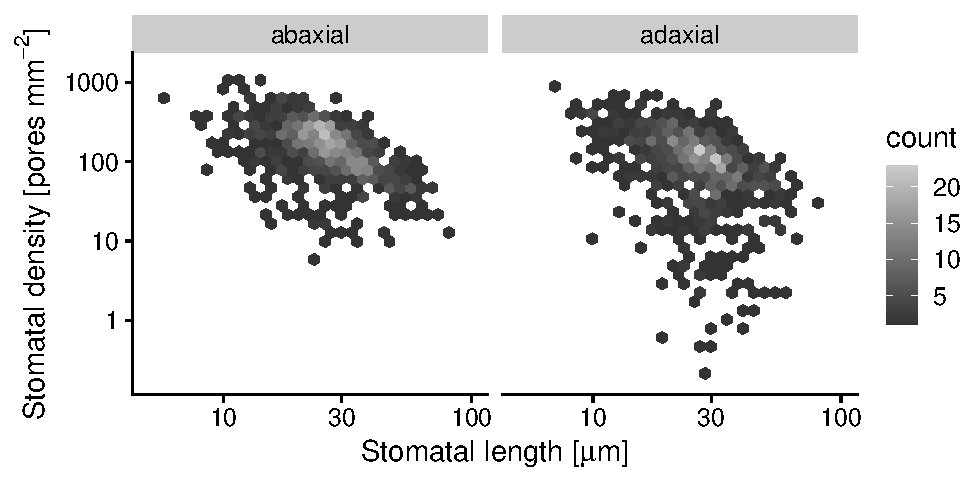
\includegraphics[width=\textwidth]{../figures/h1-raw.pdf}
\caption{Inverse size-density scaling in a synthesis of amphistomatous leaf traits across 711 taxa. The panels show the relationship between stomatal length ($x$-axis) and stomatal density ($y$-axis) on a log-log scale for values measured on the abaxial leaf surface (left) and the adaxial leaf surface (right). To avoid overplotting of points, we used a hexbin plot in which the shade of the hexagonal bin indicates the number of points in that bin. Whiter shades indicate more points (see scale to the right).}
\label{fig:h1_raw}
\end{figure}

\begin{figure}[ht]
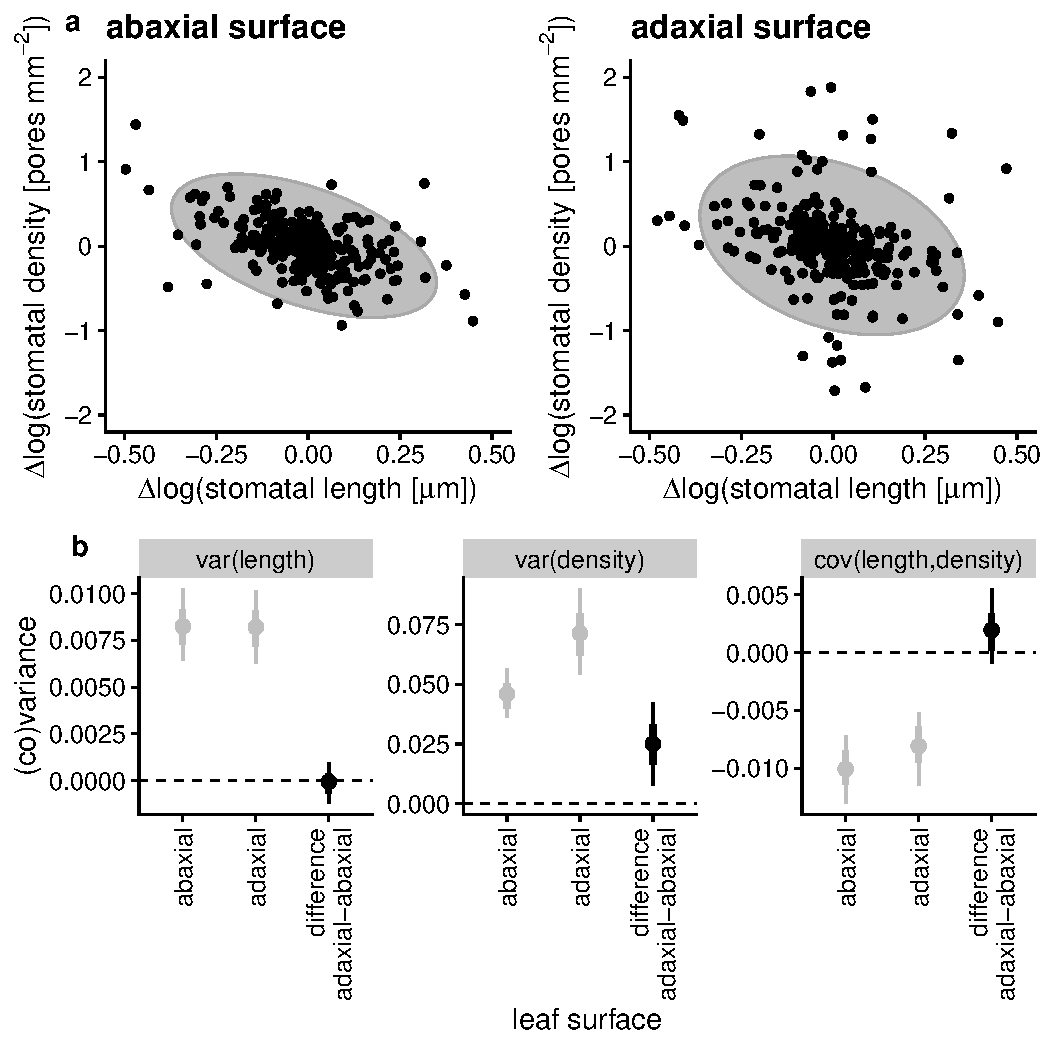
\includegraphics[width=\textwidth]{../figures/h1.pdf}
\caption{Evolutionary divergence in adaxial stomatal density is more variable, but covariance between density and length is similar on both surfaces. (a) Data from 327 phylogenetically independent contrasts of change in log(stomatal length) ($x$-axis) and log(stomatal density) ($y$-axis) for abaxial (left panel) and adaxial (right panel) leaf surfaces. Each contrast is shown by black points and every contrast appears on both panels. Grey ellipses are the model-estimated 95\% covariance ellipses. The negative covariance is similar for both surfaces but the breadth in the $y$-direction is larger for adaxial traits, indicating greater evolutionary divergence in log(stomatal density). (b) Parameter estimates (points), 66\% (thick lines), and 95\% HPD intervals for estimates of trait (co)variance. Grey points and lines represent ab- and adaxial values; black points and lines represent the estimated difference in (co)variance between surfaces. Only the variance for stomatal density (middle panel) is significantly greater for the adaxial surface (95\% HPD interval does not overlap the dashed line at 0). Reported paremeter estimates are conditioned on zero time since divergence between taxa (see \protect\hyperlink{results}{Results}).}
\label{fig:h1}
\end{figure}

\hypertarget{stomatal-density-on-each-surface-is-less-integrated-than-stomatal-length}{%
\subsection{Stomatal density on each surface is less integrated than stomatal length}\label{stomatal-density-on-each-surface-is-less-integrated-than-stomatal-length}}

The relationship between stomatal density on each leaf surface is visually more variable than that for stomatal length (Fig. \ref{fig:h2_raw}). This pattern occurs because the slope and strength of integration for stomatal density on each surface is much weaker than that for stomatal length. The SMA slope between \(\Delta \text{log}(D_\text{ad})\) and \(\Delta \text{log}(D_\text{ab})\) is less than 1 (estimated slope \(= 0.815\), 95\% HPD interval \([0.69,0.929]\)) and the strength of association is weakly positive (estimated \(r^2 = 0.131\), 95\% HPD interval \([0.0613,0.202]\); Fig. \ref{fig:h2}). In contrast, the relationship between \(\Delta \text{log}(L_\text{ad})\) and \(\Delta \text{log}(L_\text{ab})\) is isometric (estimated slope \(= 1\), 95\% HPD interval \([0.934,1.08]\)) and strongly positive (estimated \(r^2 = 0.763\), 95\% HPD interval \([0.707,0.816]\); Fig. \ref{fig:h2}).

\begin{figure}[ht]
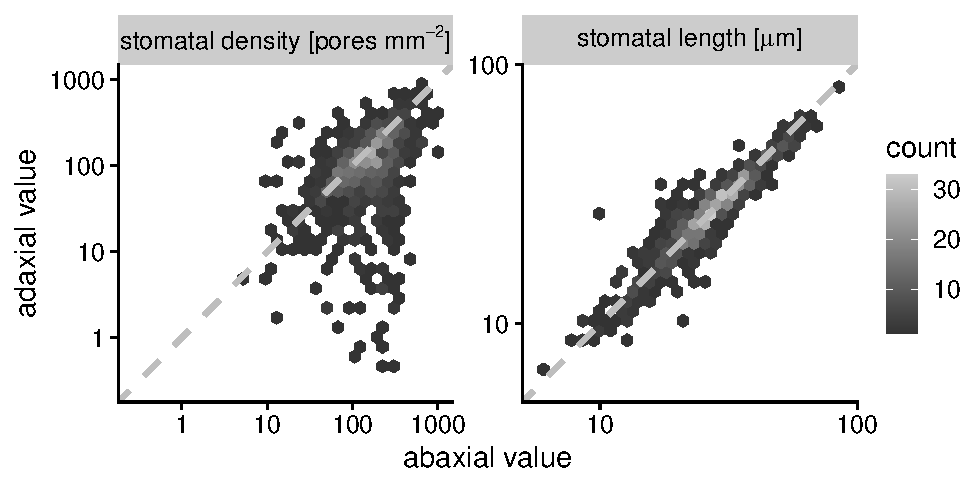
\includegraphics[width=\textwidth]{../figures/h2-raw.pdf}
\caption{Relationship stomatal density and length on each leaf surface in a synthesis of amphistomatous leaf traits across 711 taxa. The panels show the relationship between the abaxial trait value ($x$-axis) and the adaxial trait value ($y$-axis) on a log-log scale for stomatal density (left) and stomatal length (right). To avoid overplotting of points, we used a hexbin plot in which the shade of the hexagonal bin indicates the number of points in that bin. Whiter shades indicate more points (see scale to the right). The dashed line in across the middle is the 1:1 line for reference.}
\label{fig:h2_raw}
\end{figure}

\begin{figure}[ht]
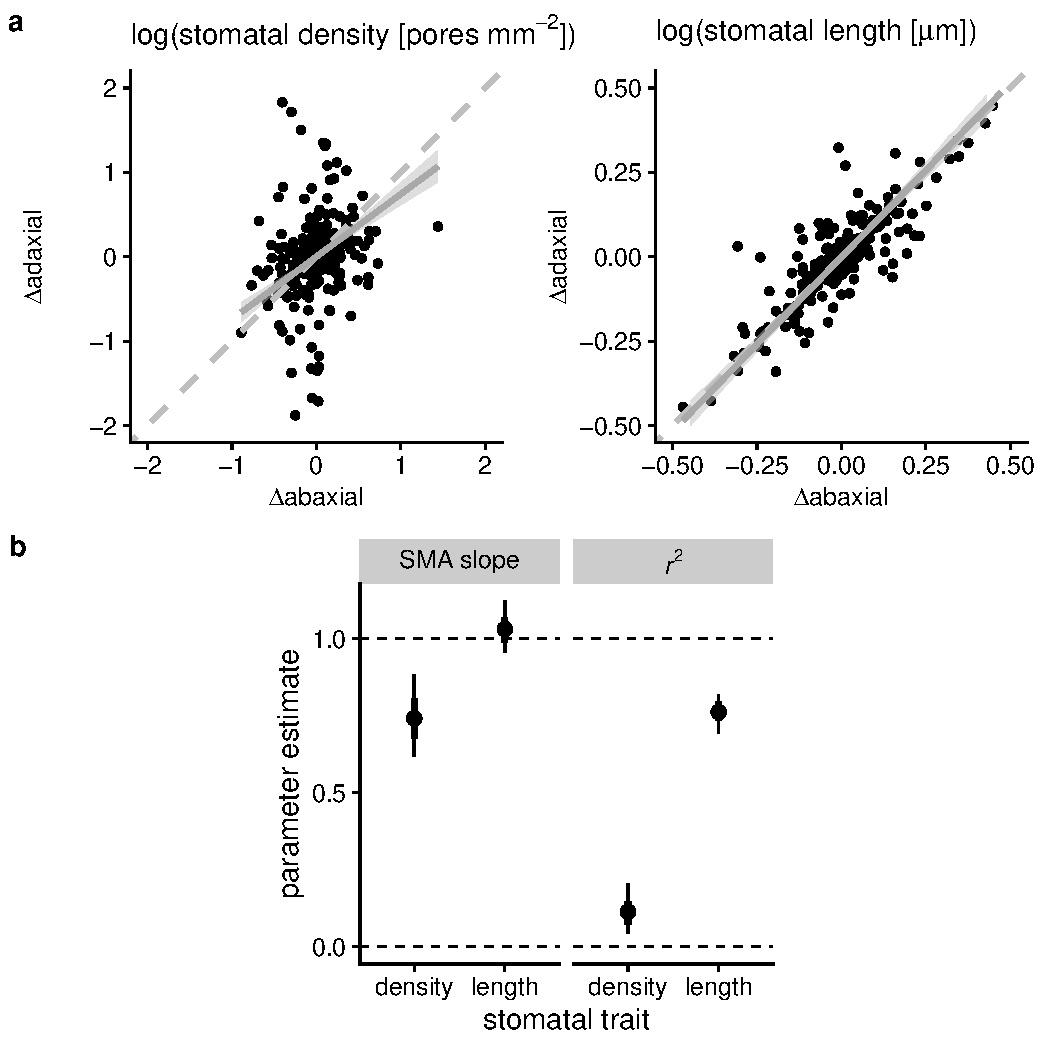
\includegraphics[width=\textwidth]{../figures/h2.pdf}
\caption{Developmental integration in stomatal length is much stronger than stomatal density between the surfaces of amphistomatous leaves (a) Data from 327 phylogenetically independent contrasts of change in the abaxial trait value ($x$-axis) against change in the adaxial trait value ($y$-axis) for log(stomatal density) (left panel) and log(stomatal length) (right panel). Each contrast is shown by black points and every contrast appears on both panels. Dashed grey lines are 1:1 lines for reference. Solid grey lines and ribbon the fitted SMA slope and 95\% HPD interval. (b) The SMA slope (left panel) is significantly less than 1 (isometry, top dashed line) for density but very close to isometric for length. The coefficient of determination ($r^2$, right panel) is also much greater for length than density. The points are parameter estimates with 66\% (thick lines) and 95\% HPD intervals. Reported paremeter estimates are conditioned on zero time since divergence between taxa (see \protect\hyperlink{results}{Results}).}
\label{fig:h2}
\end{figure}

\hypertarget{discussion}{%
\section{Discussion}\label{discussion}}

Developmental integration leads to trait covariation and may hinder adaptation by preventing traits from evolving independently towards a multivariate phenotypic optimum. Two major features of stomatal anatomical variation at the macroevolutionary scale, inverse size-density scaling and bimodal stomatal ratio, may be shaped by developmental integration between pavement and guard cell size on both leaf surfaces. In this study, we took advantage of the fact that amphistomatous leaves produce stomata on both abaxial (usually lower) and adaxial (usually upper) surfaces to test predictions of developmental integration hypotheses using a global phylogenetic comparison of seed plants, albeit mostly angiosperms. Contrary to developmental integration hypotheses, adaxial stomatal density (\(D_\text{ad}\)) evolves somewhat independently of adaxial stomatal length (\(L_\text{ad}\)) and abaxial stomatal density (\(D_\text{ab}\)). Hence, inverse size-density scaling and bimodal stomatal ratio cannot be attributed entirely to developmental integration. Quasi-independent evolution of traits should enable lineages to reach their fitness optimum, implying that selection is most likely a major constraint on the variation in stomatal anatomy in seed plants. Future research should test whether developmental integration is more or less important in certain lineages and identify the mechanistic basis of developmental disintegration where it occurs on the plant tree of life.

\hypertarget{does-developmental-integration-lead-to-inverse-size-density-scaling}{%
\subsection{Does developmental integration lead to inverse size-density scaling?}\label{does-developmental-integration-lead-to-inverse-size-density-scaling}}

If stomatal size and density are both determined by meristematic cell volume (\protect\hyperlink{ref-brodribb_unified_2013}{Brodribb, Jordan, and Carpenter 2013}), then we predicted inverse size-density scaling would evolve with the same (co)variance for both ab- and adaxial leaf surfaces. Contrary to this prediction, there are many combinations of stomatal density and length found on adaxial leaf surfaces that are absent from abaxial leaf surfaces (Fig. \ref{fig:h1_raw}). In principle, the different relationship between traits on each surface could be caused by different evolutionary variance in stomatal density (\(\text{Var}[\Delta \text{log}(D_\text{ab})] \ne \text{Var}[\Delta \text{log}(D_\text{ad})]\)) and/or covariance (\(\text{Cov}[\Delta \text{log}(L_\text{ab}), \Delta \text{log}(D_\text{ab})] \ne \text{Cov}[\Delta \text{log}(L_\text{ad}), \Delta \text{log}(D_\text{ad})]\)) on each surface. However, the covariance relationship between density and length is similar on each surface, whereas the evolutionary variance in adaxial stomatal density is significantly higher than that for abaxial density (\(\text{Var}[\Delta \text{log}(D_\text{ab})] < \text{Var}[\Delta \text{log}(D_\text{ad})]\); Fig. \ref{fig:h1}). Given that the average stomatal length is usually about the same on each surface (see below), these results imply that plants can often evolve stomatal densities on each surface without a concomitant change in size.

The disintegration of stomatal size and density on adaxial leaf surfaces implies that the inverse size-density scaling on abaxial surfaces (\protect\hyperlink{ref-weiss_untersuchungen_1865}{Weiss 1865}; \protect\hyperlink{ref-franks_maximum_2009}{Franks and Beerling 2009}; \protect\hyperlink{ref-de_boer_optimal_2016}{Boer et al. 2016}; \protect\hyperlink{ref-sack_developmental_2016}{Sack and Buckley 2016}; \protect\hyperlink{ref-liu_scaling_2021}{Liu et al. 2021}) is not a developmental \emph{fait accompli}. The lability of \(D_\text{ad}\) may explain why there is so much putatively adaptive variation in the trait along light gradients (\protect\hyperlink{ref-muir_light_2018}{Muir 2018}) and in coordination with other anatomical traits that vary among precipitation habitats (\protect\hyperlink{ref-pathare_increased_2020}{Pathare, Koteyeva, and Cousins 2020}). It also suggests that the relationship between genome size and stomatal anatomy at macroevolutionary scales (\protect\hyperlink{ref-roddy_scaling_2020}{Roddy et al. 2020}) may not be causal. Genome size sets a minimum on meristematic cell volume (\protect\hyperlink{ref-simova_geometrical_2012}{Šímová and Herben 2012}), but the decoupling of size and density on the adaxial surface suggests that meristematic cell volume is probably not a strong constraint on the final size of pavement and guard cells.

\hypertarget{does-developmental-integration-lead-to-bimodal-stomatal-ratio}{%
\subsection{Does developmental integration lead to bimodal stomatal ratio?}\label{does-developmental-integration-lead-to-bimodal-stomatal-ratio}}

We predicted that if abaxial and adaxial stomata are developmentally integrated then we should observe a strong, isometric relationship between trait divergence on each surface. Consistent with this prediction, divergence in stomatal length on each surface is isometric (SMA slope \(=\) 1) and strongly associated (\(r^2 =\) 0.763; Fig. \ref{fig:h2}). In contrast, divergence in stomatal density on each surface was not isometric (SMA slope \(=\) 0.815) and much less integrated (\(r^2 =\) 0.131; Fig. \ref{fig:h2}). Since average stomatal density on each surface can evolve quasi-independently, a wide variety of stomatal ratios are developmentally possible. Leaves are not ``forced'' to deploy identical stomatal development programs on each surface. Hence, the bimodal stomatal ratio pattern (\protect\hyperlink{ref-muir_making_2015}{Muir 2015}) is unlikely to be the result of developmental integration alone.

\hypertarget{limitations-and-future-research}{%
\subsection{Limitations and future research}\label{limitations-and-future-research}}

The ability of adaxial stomatal density to evolve independently of stomatal size and abaxial stomatal density is not consistent with the hypothesis that developmental integration is the primary cause leading to inverse size-density scaling or bimodal stomatal ratio. However, there are two major limitations of this study that should be addressed in future work. First, while \(D_\text{ab}\) can diverge independently of other stomatal traits globally, we cannot rule out that developmental integration is important in some lineages. For example, Berg's rule observes that vegetative and floral traits are often developmentally integrated, but integration can be broken when selection favors flowers for specialized pollination (\protect\hyperlink{ref-berg_general_1959}{Berg 1959}, \protect\hyperlink{ref-berg_ecological_1960}{1960}; \protect\hyperlink{ref-conner_raissa_2014}{Conner and Lande 2014}). Analogously, developmental integration between stomatal anatomical traits could evolve in some lineages, due to selection or other evolutionary forces, but become less integrated in other lineages. For example, \(D_\text{ab}\) and \(D_\text{ad}\) are positively genetically correlated in \emph{Oryza} (\protect\hyperlink{ref-ishimaru_identification_2001}{Ishimaru et al. 2001}; \protect\hyperlink{ref-rae_elucidating_2006}{Rae et al. 2006}), suggesting developmental integration may contribute to low variation in stomatal ratio between species of this genus (\protect\hyperlink{ref-giuliani_coordination_2013}{Giuliani et al. 2013}). A second major limitation is that covariation in traits like stomatal length, which appear to be developmentally integrated on each surface, could be caused by other processes. For example, since stomatal size affects the speed and mechanics of stomatal closure (\protect\hyperlink{ref-drake_smaller_2013}{Drake, Froend, and Franks 2013}; \protect\hyperlink{ref-harrison_influence_2020}{Harrison et al. 2020}), there may be strong selection for similar stomatal size throughout the leaf to harmonize rates of stomatal closure. Coordination between epidermal and mesophyll development may also constrain how independently stomatal traits on each surface can evolve (\protect\hyperlink{ref-dow_disruption_2017}{Dow, Berry, and Bergmann 2017}; \protect\hyperlink{ref-lundgren_mesophyll_2019}{Lundgren et al. 2019}).

Future research should identify the mechanistic basis of developmental disintegration between \(D_\text{ab}\) and \(D_\text{ad}\). Multiple reviews of stomatal development conclude that stomatal traits are independently controlled on each surface (\protect\hyperlink{ref-lake_longdistance_2002}{Lake, Woodward, and Quick 2002}; \protect\hyperlink{ref-bergmann_stomatal_2007}{Bergmann and Sack 2007}), but we do not know much about linkage between ab-adaxial polarity and stomatal development (\protect\hyperlink{ref-kidner_signaling_2010}{Kidner and Timmermans 2010}; \protect\hyperlink{ref-pillitteri_mechanisms_2012}{Pillitteri and Torii 2012}). Systems that have natural variation in stomatal ratio should allow us to study how developmental disintegration evolves. Quantitative genetic studies in \emph{Brassica oleracea} L., \emph{Oryza sativa} L., \emph{Populus trichocarpa} Torr. \& A. Gray ex Hook., \emph{Populus} interspecific crosses, and \emph{Solanum} interspecific crosses, typically find partial independence of \(D_\text{ab}\) and \(D_\text{ad}\); some loci affect both traits, but some loci only affect density on one surface and/or genetic correlations are weak (\protect\hyperlink{ref-ishimaru_identification_2001}{Ishimaru et al. 2001}; \protect\hyperlink{ref-ferris_leaf_2002}{Ferris et al. 2002}; \protect\hyperlink{ref-hall_relationships_2005}{Hall et al. 2005}; \protect\hyperlink{ref-rae_elucidating_2006}{Rae et al. 2006}; \protect\hyperlink{ref-laza_quantitative_2010}{Laza et al. 2010}; \protect\hyperlink{ref-chitwood_quantitative_2013}{Chitwood et al. 2013}; \protect\hyperlink{ref-mckown_association_2014}{McKown et al. 2014}; \protect\hyperlink{ref-muir_quantitative_2014}{Muir, Pease, and Moyle 2014}; \protect\hyperlink{ref-porth_evolutionary_2015}{Porth et al. 2015}; \protect\hyperlink{ref-fetter_growthdefense_2021}{Fetter, Nelson, and Keller 2021}). For example, \emph{Populus trichocarpa} populations have putatively adaptive genetic variation in \(D_\text{ad}\). Populations are more amphistomatous at Northern latitudes with shorter growing seasons that may select for faster carbon assimilation (\protect\hyperlink{ref-mckown_association_2014}{McKown et al. 2014}; \protect\hyperlink{ref-kaluthota_higher_2015}{Kaluthota et al. 2015}; \protect\hyperlink{ref-porth_evolutionary_2015}{Porth et al. 2015}). Genetic variation in key stomatal development transcription factors is associated with latitudinal variation in \(D_\text{ad}\), which should help reveal mechanistic basis of developmental disintegration between surfaces (\protect\hyperlink{ref-mckown_role_2019}{McKown et al. 2019}).

\hypertarget{acknowledgements}{%
\section{Acknowledgements}\label{acknowledgements}}

We thank Jacob Watts for comments on earlier versions of this manuscript.

\hypertarget{author-contribution}{%
\section{Author Contribution}\label{author-contribution}}

CDM designed the study, compiled data, analyzed data, and wrote the manuscript with input from all authors. All authors contributed data.

\hypertarget{data-avaibility}{%
\section{Data avaibility}\label{data-avaibility}}

The final data set and phylogeny used in the analysis are included in the \protect\hyperlink{supporting-information}{Supporting Information}. The raw anatomical data and source code will be archived on Zenodo upon publication.

\clearpage

\hypertarget{supporting-information}{%
\section{Supporting Information}\label{supporting-information}}

\renewcommand\thefigure{S\arabic{figure}}    
\renewcommand\thetable{S\arabic{table}}    
\setcounter{figure}{0}    
\setcounter{table}{0}

\textbf{Note S1:} Final fully resolved bifurcating phylogenetic tree of 711 taxa in Newick format.

\begin{longtable}[]{@{}ll@{}}
\caption{\label{tab:sources}Primary sources of stomatal anatomical data and the taxa covered by each source.}\tabularnewline
\toprule
Source & Taxa \\
\midrule
\endfirsthead
\toprule
Source & Taxa \\
\midrule
\endhead
\protect\hyperlink{ref-arambarri_taxonomy_2005}{Arambarri et al.} (\protect\hyperlink{ref-arambarri_taxonomy_2005}{2005}) & lotus \\
\protect\hyperlink{ref-avita_structure_1980}{Avita and Inamdar} (\protect\hyperlink{ref-avita_structure_1980}{1980}) & ranunculaceae,paeoniaceae \\
\protect\hyperlink{ref-bucher_stomatal_2017}{Bucher et al.} (\protect\hyperlink{ref-bucher_stomatal_2017}{2017}) & many \\
\protect\hyperlink{ref-caldera_effects_2017}{Caldera et al.} (\protect\hyperlink{ref-caldera_effects_2017}{2017}) & arabidopsis thali,ana \\
\protect\hyperlink{ref-chandra_epidermal_1967}{Chandra} (\protect\hyperlink{ref-chandra_epidermal_1967}{1967}) & solanum \\
\protect\hyperlink{ref-conesa_stomatal_2019}{Conesa et al.} (\protect\hyperlink{ref-conesa_stomatal_2019}{2019}) & limonium \\
\protect\hyperlink{ref-eckerson_number_1908}{Eckerson} (\protect\hyperlink{ref-eckerson_number_1908}{1908}) & many \\
\protect\hyperlink{ref-gindel_stomatal_1969}{Gindel} (\protect\hyperlink{ref-gindel_stomatal_1969}{1969}) & many \\
\protect\hyperlink{ref-giuliani_coordination_2013}{Giuliani et al.} (\protect\hyperlink{ref-giuliani_coordination_2013}{2013}) & oryza \\
\protect\hyperlink{ref-hanafy_leaf_2019}{Hanafy et al.} (\protect\hyperlink{ref-hanafy_leaf_2019}{2019}) & mentha \\
\protect\hyperlink{ref-huang_leaf_2019}{Huang} (\protect\hyperlink{ref-huang_leaf_2019}{2019}) & trees \\
\protect\hyperlink{ref-juhasz_effect_1966}{Juhász} (\protect\hyperlink{ref-juhasz_effect_1966}{1966}) & solanum \\
\protect\hyperlink{ref-juhasz_comparative_1968}{Juhász} (\protect\hyperlink{ref-juhasz_comparative_1968}{1968}) & solanum \\
\protect\hyperlink{ref-kannabiran_foliar_1988}{Kannabiran and Ramassamy} (\protect\hyperlink{ref-kannabiran_foliar_1988}{1988}) & apocynaceae \\
\protect\hyperlink{ref-kawamitsu_stomatal_1996}{Kawamitsu et al.} (\protect\hyperlink{ref-kawamitsu_stomatal_1996}{1996}) & grasses \\
\protect\hyperlink{ref-khan_taxonomic_2019}{Khan et al.} (\protect\hyperlink{ref-khan_taxonomic_2019}{2019}) & gymnosperms \\
\protect\hyperlink{ref-kim_comparative_1987}{Kim} (\protect\hyperlink{ref-kim_comparative_1987}{1987}) & silverswords \\
\protect\hyperlink{ref-mckown_trait_2016}{McKown, Akamine, and Sack} (\protect\hyperlink{ref-mckown_trait_2016}{2016}) & scaevola \\
\protect\hyperlink{ref-muir_unpublished_2021}{Muir, Galmés, and Conesa} (\protect\hyperlink{ref-muir_unpublished_2021}{2021}) & solanum \\
\protect\hyperlink{ref-pallardy_frequency_1979}{Pallardy and Kozlowski} (\protect\hyperlink{ref-pallardy_frequency_1979}{1979}) & populus \\
\protect\hyperlink{ref-pandey_patterns_2003}{Pandey and Nagar} (\protect\hyperlink{ref-pandey_patterns_2003}{2003}) & many \\
\protect\hyperlink{ref-pathare_increased_2020}{Pathare, Koteyeva, and Cousins} (\protect\hyperlink{ref-pathare_increased_2020}{2020}) & grasses \\
\protect\hyperlink{ref-rivera_meso-_2017}{Rivera, Villaseñor, and Terrazas} (\protect\hyperlink{ref-rivera_meso-_2017}{2017}) & asteraceae \\
\protect\hyperlink{ref-rodriguez_unpublished_2021}{Rodriguez} (\protect\hyperlink{ref-rodriguez_unpublished_2021}{2021}) & eucalyptus \\
\protect\hyperlink{ref-scalon_leaf_2016}{Scalon et al.} (\protect\hyperlink{ref-scalon_leaf_2016}{2016}) & passovia \\
\protect\hyperlink{ref-siddiqi_contribution_1991}{Siddiqi, Ahmad, and Rehman} (\protect\hyperlink{ref-siddiqi_contribution_1991}{1991}) & euphorbiaceae \\
\protect\hyperlink{ref-sporck_hawaiian_2011}{Sporck} (\protect\hyperlink{ref-sporck_hawaiian_2011}{2011}) & euphorbia \\
\protect\hyperlink{ref-stenglein_leaf_2003}{Stenglein et al.} (\protect\hyperlink{ref-stenglein_leaf_2003}{2003a}) & lotus \\
\protect\hyperlink{ref-stenglein_leaf_2003-1}{Stenglein et al.} (\protect\hyperlink{ref-stenglein_leaf_2003-1}{2003b}) & lotus \\
\protect\hyperlink{ref-sundberg_comparison_1986}{Sundberg} (\protect\hyperlink{ref-sundberg_comparison_1986}{1986}) & many \\
\protect\hyperlink{ref-szymura_leaf_2011}{Szymura and Wolski} (\protect\hyperlink{ref-szymura_leaf_2011}{2011}) & solidago \\
\protect\hyperlink{ref-xiong_one_2020}{Xiong and Flexas} (\protect\hyperlink{ref-xiong_one_2020}{2020}) & many \\
\protect\hyperlink{ref-yang_large-scale_2014}{Yang et al.} (\protect\hyperlink{ref-yang_large-scale_2014}{2014}) & many \\
\protect\hyperlink{ref-zarinkamar_density_2006}{Zarinkamar} (\protect\hyperlink{ref-zarinkamar_density_2006}{2006}) & monocots \\
\protect\hyperlink{ref-zarinkamar_stomatal_2007}{Zarinkamar} (\protect\hyperlink{ref-zarinkamar_stomatal_2007}{2007}) & eudicots \\
\protect\hyperlink{ref-zhao_difference_2020}{Zhao et al.} (\protect\hyperlink{ref-zhao_difference_2020}{2020}) & monocots \\
\protect\hyperlink{ref-zlatkovic_epidermal_2017}{Zlatković et al.} (\protect\hyperlink{ref-zlatkovic_epidermal_2017}{2017}) & sedum \\
\protect\hyperlink{ref-zoric_leaf_2009}{Zoric et al.} (\protect\hyperlink{ref-zoric_leaf_2009}{2009}) & trifolium \\
\bottomrule
\end{longtable}

\clearpage

\begin{table}
\caption{\label{tab:pair_div}Final data set of 327 taxon pairs for analysis. $\tt{tree\_node}$ is the node of the common ancestor of the taxon pair $\tt{sp1}$ and $\tt{sp2}$ in the phylogeny (Note S1). $\tt{pair\_age}$ is the time in millions of years since taxa split. The remaining columns are the trait divergence (log-scale) between taxa ($\Delta \text{log(trait)}$).}
\end{table}

\begin{table}[ht]
\caption{\label{tab:modeloutput} Parameter estimates and 95\% highest posterior density (HPD) intervals. For each trait ($D_\mathrm{ab}$, $D_\mathrm{ad}$, $L_\mathrm{ab}$, $L_\mathrm{ad}$) we estimated the average (median) divergence between taxon pairs, denoted $\Delta \text{log(trait)}$. See Table \ref{tab:traits} for symbol definitions. The second section is the standard deviation of $\Delta \text{log(trait)}$. The third section is the estimated coefficient of pair age (millions of years) on the standard devition on a log-link scale. The fourth section is the estimated correlation coefficient between $\Delta \text{log(trait)}$ of all pairwise trait combinations. The final section is the estimated $\nu$ family of the Student $t$ distribution.}
\begin{center}
\begin{tabular}{lll}

  \toprule
  Trait(s) & Estimate & 95\% HPD interval \\
  \midrule
  
  \multicolumn{3}{l}{Average $\Delta \text{log(trait)}$} \\
  \\
  $D_\mathrm{ab}$ & -0.0015  & $-0.03-0.031$  \\
  $D_\mathrm{ad}$ & -0.0019  & $-0.04-0.038$  \\
  $L_\mathrm{ab}$ & -0.0038  & $-0.016-0.0096$  \\
  $L_\mathrm{ad}$ & -0.0017  & $-0.015-0.011$  \\
  \\
  \multicolumn{3}{l}{Standard deviation of $\Delta \text{log(trait)}$} \\
  \\
  $D_\mathrm{ab}$ & 0.230  & $0.2-0.26$  \\
  $D_\mathrm{ad}$ & 0.280  & $0.24-0.32$  \\
  $L_\mathrm{ab}$ & 0.094  & $0.083-0.1$  \\
  $L_\mathrm{ad}$ & 0.094  & $0.084-0.11$  \\
  \\
  \multicolumn{3}{l}{Effect of pair age on standard deviation of $\Delta \text{log(trait)}$} \\
  \multicolumn{3}{l}{log-link scale} \\
  \\
  $D_\mathrm{ab}$ & 0.0098  & $0.0039-0.017$  \\
  $D_\mathrm{ad}$ & 0.0170  & $0.01-0.024$  \\
  $L_\mathrm{ab}$ & 0.0140  & $0.0091-0.02$  \\
  $L_\mathrm{ad}$ & 0.0150  & $0.0096-0.021$  \\
  \\
  \multicolumn{3}{l}{Correlation between $\Delta \text{log(trait)}$} \\
  \\
  $D_\mathrm{ab}-D_\mathrm{ad}$ & 
   0.36  & $0.26-0.46$  \\
  $D_\mathrm{ab}-L_\mathrm{ab}$ & 
  -0.55  & $-0.63--0.47$  \\
  $D_\mathrm{ab}-L_\mathrm{ad}$ & 
  -0.43  & $-0.53--0.34$  \\
  $D_\mathrm{ad}-L_\mathrm{ab}$ & 
  -0.31  & $-0.41--0.2$  \\
  $D_\mathrm{ad}-L_\mathrm{ad}$ & 
  -0.34  & $-0.45--0.24$  \\
  $L_\mathrm{ab}-L_\mathrm{ad}$ & 
   0.87  & $0.84-0.9$  \\
  \\
  \multicolumn{3}{l}{Student $t$ famil parameter $\nu$} \\
  \\
  $-$ & 3.7  & $2.8-4.7$  \\

\bottomrule

\end{tabular}
\end{center}
\end{table}

\clearpage

\hypertarget{references}{%
\section*{References}\label{references}}
\addcontentsline{toc}{section}{References}

\hypertarget{refs}{}
\begin{CSLReferences}{1}{0}
\leavevmode\hypertarget{ref-anderson_diverge_2021}{}%
Anderson, Sean A S, and Jason T Weir. 2021. \emph{Diverge: {Evolutionary} {Trait} {Divergence} {Between} {Sister} {Species} and {Other} {Paired} {Lineages}}. \url{https://CRAN.R-project.org/package=diverge}.

\leavevmode\hypertarget{ref-arambarri_taxonomy_2005}{}%
Arambarri, Ana M., Sebastián A. Stenglein, Marta N. Colares, and María C. Novoa. 2005. {``Taxonomy of the {New} {World} Species of {Lotus} ({Leguminosae}: {Loteae}).''} \emph{Australian Journal of Botany} 53 (8): 797. \url{https://doi.org/10.1071/BT04101}.

\leavevmode\hypertarget{ref-armbruster_covariance_1999}{}%
Armbruster, W. Scott, Vero´nica S. Di Stilio, John D. Tuxill, T. Christopher Flores, and Julie L. Vela´squez Runk. 1999. {``Covariance and Decoupling of Floral and Vegetative Traits in Nine {Neotropical} Plants: A Re‐evaluation of {Berg}'s Correlation‐pleiades Concept.''} \emph{American Journal of Botany} 86 (1): 39--55. \url{https://doi.org/10.2307/2656953}.

\leavevmode\hypertarget{ref-armbruster_integrated_2014}{}%
Armbruster, W. Scott, Christophe Pélabon, Geir H. Bolstad, and Thomas F. Hansen. 2014. {``Integrated Phenotypes: Understanding Trait Covariation in Plants and Animals.''} \emph{Philosophical Transactions of the Royal Society B: Biological Sciences} 369 (1649): 20130245. \url{https://doi.org/10.1098/rstb.2013.0245}.

\leavevmode\hypertarget{ref-avita_structure_1980}{}%
Avita, S. R., and J. A. Inamdar. 1980. {``Structure and {Ontogeny} of {Stomata} in {Ranunculaceae} and {Paeoniaceae}.''} \emph{Flora} 170 (4): 354--70. \url{https://doi.org/10.1016/S0367-2530(17)31224-0}.

\leavevmode\hypertarget{ref-barrett_sexual_2013}{}%
Barrett, Spencer C. H., and Josh Hough. 2013. {``Sexual Dimorphism in Flowering Plants.''} \emph{Journal of Experimental Botany} 64 (1): 67--82. \url{https://doi.org/10.1093/jxb/ers308}.

\leavevmode\hypertarget{ref-berg_general_1959}{}%
Berg, R. L. 1959. {``A {General} {Evolutionary} {Principle} {Underlying} the {Origin} of {Developmental} {Homeostasis}.''} \emph{The American Naturalist} 93 (869): 103--5. \url{https://doi.org/10.1086/282061}.

\leavevmode\hypertarget{ref-berg_ecological_1960}{}%
---------. 1960. {``The {Ecological} {Significance} of {Correlation} {Pleiades}.''} \emph{Evolution} 14 (2): 171. \url{https://doi.org/10.2307/2405824}.

\leavevmode\hypertarget{ref-bergmann_stomatal_2007}{}%
Bergmann, Dominique C., and Fred D. Sack. 2007. {``Stomatal {Development}.''} \emph{Annual Review of Plant Biology} 58 (1): 163--81. \url{https://doi.org/10.1146/annurev.arplant.58.032806.104023}.

\leavevmode\hypertarget{ref-de_boer_optimal_2016}{}%
Boer, Hugo J de, Charles A Price, Friederike Wagner‐Cremer, Stefan C Dekker, Peter J Franks, and Erik J Veneklaas. 2016. {``Optimal Allocation of Leaf Epidermal Area for Gas Exchange.''} \emph{New Phytologist} 210 (4): 1219--28. \url{https://doi.org/10.1111/nph.13929}.

\leavevmode\hypertarget{ref-brodribb_unified_2013}{}%
Brodribb, Tim J., Greg J. Jordan, and Raymond J. Carpenter. 2013. {``Unified Changes in Cell Size Permit Coordinated Leaf Evolution.''} \emph{New Phytologist} 199 (2): 559--70. \url{https://doi.org/10.1111/nph.12300}.

\leavevmode\hypertarget{ref-bucher_stomatal_2017}{}%
Bucher, Solveig Franziska, Karl Auerswald, Christina Grün-Wenzel, Steven I. Higgins, Javier Garcia Jorge, and Christine Römermann. 2017. {``Stomatal Traits Relate to Habitat Preferences of Herbaceous Species in a Temperate Climate.''} \emph{Flora} 229 (April): 107--15. \url{https://doi.org/10.1016/j.flora.2017.02.011}.

\leavevmode\hypertarget{ref-buckley_how_2015}{}%
Buckley, Thomas N., Grace P. John, Christine Scoffoni, and Lawren Sack. 2015. {``How {Does} {Leaf} {Anatomy} {Influence} {Water} {Transport} Outside the {Xylem}?''} \emph{Plant Physiology} 168 (4): 1616--35. \url{https://doi.org/10.1104/pp.15.00731}.

\leavevmode\hypertarget{ref-burkner_brms_2017}{}%
Bürkner, Paul-Christian. 2017. {``\textbf{Brms} : {An} \emph{r} {Package} for {Bayesian} {Multilevel} {Models} {Using} \emph{Stan}.''} \emph{Journal of Statistical Software} 80 (1). \url{https://doi.org/10.18637/jss.v080.i01}.

\leavevmode\hypertarget{ref-burkner_advanced_2018}{}%
---------. 2018. {``Advanced {Bayesian} {Multilevel} {Modeling} with the {R} {Package} Brms.''} \emph{The R Journal} 10 (1): 395. \url{https://doi.org/10.32614/RJ-2018-017}.

\leavevmode\hypertarget{ref-caldera_effects_2017}{}%
Caldera, H. Iroja U., W. A. Janendra M. De Costa, F. Ian Woodward, Janice A. Lake, and Sudheera M. W. Ranwala. 2017. {``Effects of Elevated Carbon Dioxide on Stomatal Characteristics and Carbon Isotope Ratio of \emph{{Arabidopsis} Thaliana} Ecotypes Originating from an Altitudinal Gradient.''} \emph{Physiologia Plantarum} 159 (1): 74--92. \url{https://doi.org/10.1111/ppl.12486}.

\leavevmode\hypertarget{ref-chamberlain_taxize_2013}{}%
Chamberlain, Scott A., and Eduard Szöcs. 2013. {``Taxize: Taxonomic Search and Retrieval in {R}.''} \emph{F1000Research} 2 (October): 191. \url{https://doi.org/10.12688/f1000research.2-191.v2}.

\leavevmode\hypertarget{ref-chandra_epidermal_1967}{}%
Chandra, V. 1967. {``Epidermal Studies on Some {Solanaceous} Plants.''} \emph{Indian Journal of Pharmacy} 29: 227--29.

\leavevmode\hypertarget{ref-chitwood_quantitative_2013}{}%
Chitwood, Daniel H, Ravi Kumar, Lauren R Headland, Aashish Ranjan, Michael F Covington, Yasunori Ichihashi, Daniel Fulop, et al. 2013. {``A Quantitative Genetic Basis for Leaf Morphology in a Set of Precisely Defined Tomato Introgression Lines.''} \emph{The Plant Cell} 25 (7): 2465--81.

\leavevmode\hypertarget{ref-conesa_stomatal_2019}{}%
Conesa, Miquel À, Christopher D Muir, Arantzazu Molins, and Jeroni Galmés. 2019. {``Stomatal Anatomy Coordinates Leaf Size with {Rubisco} Kinetics in the {Balearic} {Limonium}.''} \emph{AoB PLANTS}, August, plz050. \url{https://doi.org/10.1093/aobpla/plz050}.

\leavevmode\hypertarget{ref-conner_raissa_2014}{}%
Conner, Jeffrey K., and Russell Lande. 2014. {``Raissa {L}. {Berg}'s Contributions to the Study of Phenotypic Integration, with a Professional Biographical Sketch.''} \emph{Philosophical Transactions of the Royal Society B: Biological Sciences} 369 (1649): 20130250. \url{https://doi.org/10.1098/rstb.2013.0250}.

\leavevmode\hypertarget{ref-deans_optimization_2020}{}%
Deans, Ross M., Timothy J. Brodribb, Florian A. Busch, and Graham D. Farquhar. 2020. {``Optimization Can Provide the Fundamental Link Between Leaf Photosynthesis, Gas Exchange and Water Relations.''} \emph{Nature Plants} 6 (9): 1116--25. \url{https://doi.org/10.1038/s41477-020-00760-6}.

\leavevmode\hypertarget{ref-dow_disruption_2017}{}%
Dow, Graham J., Joseph A. Berry, and Dominique C. Bergmann. 2017. {``Disruption of Stomatal Lineage Signaling or Transcriptional Regulators Has Differential Effects on Mesophyll Development, but Maintains Coordination of Gas Exchange.''} \emph{New Phytologist} 216 (1): 69--75. \url{https://doi.org/10.1111/nph.14746}.

\leavevmode\hypertarget{ref-drake_two_2019}{}%
Drake, Paul L., Hugo J. de Boer, Stanislaus J. Schymanski, and Erik J. Veneklaas. 2019. {``Two Sides to Every Leaf: Water and {CO}\(_{\textrm{2}}\) Transport in Hypostomatous and Amphistomatous Leaves.''} \emph{New Phytologist} 222 (3): 1179--87. \url{https://doi.org/10.1111/nph.15652}.

\leavevmode\hypertarget{ref-drake_smaller_2013}{}%
Drake, Paul L., Ray H Froend, and Peter J Franks. 2013. {``Smaller, Faster Stomata: Scaling of Stomatal Size, Rate of Response, and Stomatal Conductance.''} \emph{Journal of Experimental Botany} 64 (2): 495--505. \url{https://doi.org/10.1093/jxb/ers347}.

\leavevmode\hypertarget{ref-eckerson_number_1908}{}%
Eckerson, Sophia H. 1908. {``The Number and Size of the Stomata.''} \emph{Botanical Gazette} 46 (3): 221--24.

\leavevmode\hypertarget{ref-felsenstein_phylogenies_1985}{}%
Felsenstein, Joseph. 1985. {``Phylogenies and the Comparative Method.''} \emph{The American Naturalist} 1 (125): 1--15.

\leavevmode\hypertarget{ref-ferris_leaf_2002}{}%
Ferris, R., L. Long, S. M. Bunn, K. M. Robinson, H. D. Bradshaw, A. M. Rae, and G. Taylor. 2002. {``Leaf Stomatal and Epidermal Cell Development: Identification of Putative Quantitative Trait Loci in Relation to Elevated Carbon Dioxide Concentration in Poplar.''} \emph{Tree Physiology} 22 (9): 633--40. \url{https://doi.org/10.1093/treephys/22.9.633}.

\leavevmode\hypertarget{ref-fetter_growthdefense_2021}{}%
Fetter, Karl C., David M. Nelson, and Stephen R. Keller. 2021. {``Growth‐defense Trade‐offs Masked in Unadmixed Populations Are Revealed by Hybridization.''} \emph{Evolution} 75 (6): 1450--65. \url{https://doi.org/10.1111/evo.14227}.

\leavevmode\hypertarget{ref-franks_maximum_2009}{}%
Franks, Peter J, and David J Beerling. 2009. {``Maximum Leaf Conductance Driven by {CO}\(_{\textrm{2}}\) Effects on Stomatal Size and Density over Geologic Time.''} \emph{Proceedings of the National Academy of Sciences} 106 (25): 10343--47.

\leavevmode\hypertarget{ref-franks_effect_2001}{}%
Franks, Peter J, and Graham D Farquhar. 2001. {``The {Effect} of {Exogenous} {Abscisic} {Acid} on {Stomatal} {Development}, {Stomatal} {Mechanics}, and {Leaf} {Gas} {Exchange} in \emph{{Tradescantia} Virginiana}.''} \emph{Plant Physiology} 125 (2): 935--42. \url{https://doi.org/10.1104/pp.125.2.935}.

\leavevmode\hypertarget{ref-gabry_cmdstanr_2021}{}%
Gabry, Jonah, and Rok Češnovar. 2021. \emph{Cmdstanr: {R} {Interface} to '{CmdStan}'}. \url{https://mc-stan.org/cmdstanr,\%20https://discourse.mc-stan.org}.

\leavevmode\hypertarget{ref-galmes_leaf_2013}{}%
Galmés, Jeroni, Joan Manuel Ochogavía, Jorge Gago, Emilio José Roldán, Josep Cifre, and Miquel Àngel Conesa. 2013. {``Leaf Responses to Drought Stress in {Mediterranean} Accessions of {Solanum} Lycopersicum: Anatomical Adaptations in Relation to Gas Exchange Parameters.''} \emph{Plant, Cell \& Environment} 36 (5): 920--35. \url{https://doi.org/10.1111/pce.12022}.

\leavevmode\hypertarget{ref-gibson_structure-function_1996}{}%
Gibson, Arthur C. 1996. \emph{Structure-{Function} {Relations} of {Warm} {Desert} {Plants}}. Berlin, Heidelberg: Springer Berlin / Heidelberg. \url{http://public.eblib.com/choice/PublicFullRecord.aspx?p=6495247}.

\leavevmode\hypertarget{ref-gindel_stomatal_1969}{}%
Gindel, I. 1969. {``Stomatal Number and Size as Related to Soil Moisture in Tree Xerophytes in {Israel}.''} \emph{Ecology} 50 (2): 263--67.

\leavevmode\hypertarget{ref-giuliani_coordination_2013}{}%
Giuliani, R., N. Koteyeva, E. Voznesenskaya, M. A. Evans, A. B. Cousins, and G. E. Edwards. 2013. {``Coordination of {Leaf} {Photosynthesis}, {Transpiration}, and {Structural} {Traits} in {Rice} and {Wild} {Relatives} ({Genus} {Oryza}).''} \emph{PLANT PHYSIOLOGY} 162 (3): 1632--51. \url{https://doi.org/10.1104/pp.113.217497}.

\leavevmode\hypertarget{ref-gutschick_photosynthesis_1984}{}%
Gutschick, Vincent P. 1984. {``Photosynthesis Model for {C}\(_{\textrm{3}}\) Leaves Incorporating {CO}\(_{\textrm{2}}\) Transport, Propagation of Radiation, and Biochemistry 2. Ecological and Agricultural Utility.''} \emph{Photosynthetica} 18 (4): 569--95.

\leavevmode\hypertarget{ref-hall_relationships_2005}{}%
Hall, N. M., H. Griffiths, J. A. Corlett, H. G. Jones, J. Lynn, and G. J. King. 2005. {``Relationships Between Water-Use Traits and Photosynthesis in \emph{{Brassica} Oleracea} Resolved by Quantitative Genetic Analysis.''} \emph{Plant Breeding} 124 (6): 557--64. \url{https://doi.org/10.1111/j.1439-0523.2005.01164.x}.

\leavevmode\hypertarget{ref-hanafy_leaf_2019}{}%
Hanafy, Doaa M., Paul D. Prenzler, Rodney A. Hill, and Geoffrey E. Burrows. 2019. {``Leaf Micromorphology of 19 {Mentha} Taxa.''} \emph{Australian Journal of Botany} 67 (7): 463. \url{https://doi.org/10.1071/BT19054}.

\leavevmode\hypertarget{ref-hansen_is_2003}{}%
Hansen, Thomas F. 2003. {``Is Modularity Necessary for Evolvability?''} \emph{Biosystems} 69 (2-3): 83--94. \url{https://doi.org/10.1016/S0303-2647(02)00132-6}.

\leavevmode\hypertarget{ref-harrison_influence_2020}{}%
Harrison, Emily L., Lucia Arce Cubas, Julie E. Gray, and Christopher Hepworth. 2020. {``The Influence of Stomatal Morphology and Distribution on Photosynthetic Gas Exchange.''} \emph{The Plant Journal} 101 (4): 768--79. \url{https://doi.org/10.1111/tpj.14560}.

\leavevmode\hypertarget{ref-henry_stomatal_2019}{}%
Henry, Christian, Grace P. John, Ruihua Pan, Megan K. Bartlett, Leila R. Fletcher, Christine Scoffoni, and Lawren Sack. 2019. {``A Stomatal Safety-Efficiency Trade-Off Constrains Responses to Leaf Dehydration.''} \emph{Nature Communications} 10 (1): 3398. \url{https://doi.org/10.1038/s41467-019-11006-1}.

\leavevmode\hypertarget{ref-huang_leaf_2019}{}%
Huang, Sophia. 2019. {``Leaf Functional Traits as Predictors of Drought Tolerance in Urban Trees.''} Master's thesis, San Luis Obispo: California Polytechnic State University, San Luis Obispo.

\leavevmode\hypertarget{ref-ishimaru_identification_2001}{}%
Ishimaru, Ken, Kanako Shirota, Masae Higa, and Yoshinobu Kawamitsu. 2001. {``Identification of Quantitative Trait Loci for Adaxial and Abaxial Stomatal Frequencies in \emph{{Oryza} Sativa}.''} \emph{Plant Physiology and Biochemistry} 39 (2): 173--77. \url{https://doi.org/10.1016/S0981-9428(00)01232-8}.

\leavevmode\hypertarget{ref-jin_vphylomaker_2019}{}%
Jin, Yi, and Hong Qian. 2019. {``V.{PhyloMaker}: An {R} Package That Can Generate Very Large Phylogenies for Vascular Plants.''} \emph{Ecography} 42 (8): 1353--59. \url{https://doi.org/10.1111/ecog.04434}.

\leavevmode\hypertarget{ref-jordan_using_2014}{}%
Jordan, Gregory J., Raymond J. Carpenter, and Timothy J. Brodribb. 2014. {``Using Fossil Leaves as Evidence for Open Vegetation.''} \emph{Palaeogeography, Palaeoclimatology, Palaeoecology} 395 (February): 168--75. \url{https://doi.org/10.1016/j.palaeo.2013.12.035}.

\leavevmode\hypertarget{ref-juhasz_effect_1966}{}%
Juhász, M. 1966. {``Effect of Ecological Factors on the Leaf Epidermis of Species {Solanum}.''} \emph{Acta Biologica} 12 (3-4): 29--36.

\leavevmode\hypertarget{ref-juhasz_comparative_1968}{}%
---------. 1968. {``A Comparative Histological Examination of the Leaf Epidermis of Some {Solanum} Species.''} \emph{Acta Biologica} 14: 5--9.

\leavevmode\hypertarget{ref-kaluthota_higher_2015}{}%
Kaluthota, Sobadini, David W. Pearce, Luke M. Evans, Matthew G. Letts, Thomas G. Whitham, and Stewart B. Rood. 2015. {``Higher Photosynthetic Capacity from Higher Latitude: Foliar Characteristics and Gas Exchange of Southern, Central and Northern Populations of \emph{{Populus} Angustifolia}.''} Edited by David Tissue. \emph{Tree Physiology} 35 (9): 936--48. \url{https://doi.org/10.1093/treephys/tpv069}.

\leavevmode\hypertarget{ref-kannabiran_foliar_1988}{}%
Kannabiran, B, and V Ramassamy. 1988. {``Foliar Epidermis and Taxonomy in {Apocynaceae}.''} \emph{Proceedings of the Indian Academy of Sciences} 98 (5): 409--17.

\leavevmode\hypertarget{ref-kawamitsu_stomatal_1996}{}%
Kawamitsu, Yoshinobu, Shin-ichi Hiyane, Seiichi Murayama, Akihiro Nose, and Choyu Shinjyo. 1996. {``Stomatal Frequency and Guard Cell Length in {C}\(_{\textrm{3}}\) and {C}\(_{\textrm{4}}\) Grass Species.''} \emph{Japanese Journal of Crop Science} 65 (4): 626--33.

\leavevmode\hypertarget{ref-khan_taxonomic_2019}{}%
Khan, Raees, Sheikh Zain Ul Abidin, Mushtaq Ahmad, Muhammad Zafar, Jie Liu, Lubna, Shayan Jamshed, and Ömer Kiliç. 2019. {``Taxonomic Importance of {SEM} and {LM} Foliar Epidermal Micro-Morphology: {A} Tool for Robust Identification of Gymnosperms.''} \emph{Flora} 255 (June): 42--68. \url{https://doi.org/10.1016/j.flora.2019.03.016}.

\leavevmode\hypertarget{ref-kidner_signaling_2010}{}%
Kidner, Catherine A., and Marja C. P. Timmermans. 2010. {``Signaling {Sides}.''} In \emph{Current {Topics} in {Developmental} {Biology}}, 91:141--68. Elsevier. \url{https://doi.org/10.1016/S0070-2153(10)91005-3}.

\leavevmode\hypertarget{ref-kim_comparative_1987}{}%
Kim, Insun. 1987. {``Comparative {Anatomy} of {Some} {Parents} and {Hybrids} of the {Hawaiian} {Madiinae} ({Asteraceae}).''} \emph{American Journal of Botany} 74 (8): 1224--38. \url{https://doi.org/10.2307/2444158}.

\leavevmode\hypertarget{ref-lake_longdistance_2002}{}%
Lake, Janice A., F. Ian Woodward, and W. Paul Quick. 2002. {``Long‐distance {Co2} Signalling in Plants.''} \emph{Journal of Experimental Botany} 53 (367): 183--93. \url{https://doi.org/10.1093/jexbot/53.367.183}.

\leavevmode\hypertarget{ref-lande_quantitative_1979}{}%
Lande, Russell. 1979. {``Quantitative {Genetic} {Analysis} of {Multivariate} {Evolution}, {Applied} to {Brain}: {Body} {Size} {Allometry}.''} \emph{Evolution} 33 (1): 402. \url{https://doi.org/10.2307/2407630}.

\leavevmode\hypertarget{ref-laza_quantitative_2010}{}%
Laza, Ma. Rebecca C., Motohiko Kondo, Osamu Ideta, Edward Barlaan, and Tokio Imbe. 2010. {``Quantitative Trait Loci for Stomatal Density and Size in Lowland Rice.''} \emph{Euphytica} 172 (2): 149--58. \url{https://doi.org/10.1007/s10681-009-0011-8}.

\leavevmode\hypertarget{ref-lewontin_adaptation_1978}{}%
Lewontin, Richard C. 1978. {``Adaptation.''} \emph{Scientific American} 239 (3): 212--18.

\leavevmode\hypertarget{ref-liu_scaling_2021}{}%
Liu, Congcong, Christopher D Muir, Ying Li, Li Xu, Mingxu Li, Jiahui Zhang, Hugo Jan de Boer, et al. 2021. {``Scaling Between Stomatal Size and Density in Forest Plants.''} Preprint. Plant Biology. \url{https://doi.org/10.1101/2021.04.25.441252}.

\leavevmode\hypertarget{ref-lundgren_mesophyll_2019}{}%
Lundgren, Marjorie R., Andrew Mathers, Alice L. Baillie, Jessica Dunn, Matthew J. Wilson, Lee Hunt, Radoslaw Pajor, et al. 2019. {``Mesophyll Porosity Is Modulated by the Presence of Functional Stomata.''} \emph{Nature Communications} 10 (1): 2825. \url{https://doi.org/10.1038/s41467-019-10826-5}.

\leavevmode\hypertarget{ref-mckown_trait_2016}{}%
McKown, Athena D., Michelle Elmore Akamine, and Lawren Sack. 2016. {``Trait Convergence and Diversification Arising from a Complex Evolutionary History in {Hawaiian} Species of {Scaevola}.''} \emph{Oecologia} 181 (4): 1083--1100. \url{https://doi.org/10.1007/s00442-016-3640-3}.

\leavevmode\hypertarget{ref-mckown_association_2014}{}%
McKown, Athena D., Robert D. Guy, Linda Quamme, Jaroslav Klápště, Jonathan La Mantia, C. P. Constabel, Yousry A. El-Kassaby, Richard C. Hamelin, Michael Zifkin, and M. S. Azam. 2014. {``Association Genetics, Geography and Ecophysiology Link Stomatal Patterning in \emph{{Populus} Trichocarpa} with Carbon Gain and Disease Resistance Trade-Offs.''} \emph{Molecular Ecology} 23 (23): 5771--90. \url{https://doi.org/10.1111/mec.12969}.

\leavevmode\hypertarget{ref-mckown_role_2019}{}%
McKown, Athena D., Jaroslav Klápště, Robert D. Guy, Oliver R. A. Corea, Steffi Fritsche, Jürgen Ehlting, Yousry A. El‐Kassaby, and Shawn D. Mansfield. 2019. {``A Role for \emph{SPEECHLESS} in the Integration of Leaf Stomatal Patterning with the Growth Vs Disease Trade‐off in Poplar.''} \emph{New Phytologist} 223 (4): 1888--1903. \url{https://doi.org/10.1111/nph.15911}.

\leavevmode\hypertarget{ref-metcalfe_anatomy_1950}{}%
Metcalfe, Charles Russell, and Laurence Chalk. 1950. \emph{Anatomy of the Dicotyledons, {Vols}. 1 \& 2}. First. Oxford: Oxford University Press.

\leavevmode\hypertarget{ref-missouri_botanical_garden_tropicos_2020}{}%
Missouri Botanical Garden. 2020. {``Tropicos.''} \url{https://tropicos.org}.

\leavevmode\hypertarget{ref-mott_adaptive_1982}{}%
Mott, Keith A., Arthur C. Gibson, and James W. O'Leary. 1982. {``The Adaptive Significance of Amphistomatic Leaves.''} \emph{Plant, Cell \& Environment} 5 (6): 455--60. \url{https://doi.org/10.1111/1365-3040.ep11611750}.

\leavevmode\hypertarget{ref-muir_making_2015}{}%
Muir, Christopher D. 2015. {``Making Pore Choices: Repeated Regime Shifts in Stomatal Ratio.''} \emph{Proceedings of the Royal Society B: Biological Sciences} 282 (1813): 20151498. \url{https://doi.org/10.1098/rspb.2015.1498}.

\leavevmode\hypertarget{ref-muir_light_2018}{}%
---------. 2018. {``Light and Growth Form Interact to Shape Stomatal Ratio Among {British} Angiosperms.''} \emph{New Phytologist} 218 (1): 242--52.

\leavevmode\hypertarget{ref-muir_is_2019}{}%
---------. 2019. {``Is {Amphistomy} an {Adaptation} to {High} {Light}? {Optimality} {Models} of {Stomatal} {Traits} Along {Light} {Gradients}.''} \emph{Integrative and Comparative Biology} 59 (3): 571--84. \url{https://doi.org/10.1093/icb/icz085}.

\leavevmode\hypertarget{ref-muir_unpublished_2021}{}%
Muir, Christopher D, Jeroni Galmés, and Miquel À Conesa. 2021. {``Unpublished Data.''}

\leavevmode\hypertarget{ref-muir_quantitative_2014}{}%
Muir, Christopher D, James B Pease, and Leonie C Moyle. 2014. {``Quantitative {Genetic} {Analysis} {Indicates} {Natural} {Selection} on {Leaf} {Phenotypes} {Across} {Wild} {Tomato} {Species} (\emph{Solanum} Sect. \emph{Lycopersicon} ; {Solanaceae}).''} \emph{Genetics} 198 (4): 1629--43. \url{https://doi.org/10.1534/genetics.114.169276}.

\leavevmode\hypertarget{ref-murray_consistent_2020}{}%
Murray, Michelle, Wuu Kuang Soh, Charilaos Yiotis, Robert A. Spicer, Tracy Lawson, and Jennifer C. McElwain. 2020. {``Consistent {Relationship} Between {Field}-{Measured} {Stomatal} {Conductance} and {Theoretical} {Maximum} {Stomatal} {Conductance} in {C} \(_{\textrm{3}}\) {Woody} {Angiosperms} in {Four} {Major} {Biomes}.''} \emph{International Journal of Plant Sciences} 181 (1): 142--54. \url{https://doi.org/10.1086/706260}.

\leavevmode\hypertarget{ref-ouellette_database_1997}{}%
Ouellette, B. F. Francis, and Mark S. Boguski. 1997. {``Database {Divisions} and {Homology} {Search} {Files}: {A} {Guide} for the {Perplexed}.''} \emph{Genome Research} 7 (10): 952--55. \url{https://doi.org/10.1101/gr.7.10.952}.

\leavevmode\hypertarget{ref-pallardy_frequency_1979}{}%
Pallardy, S G, and T T Kozlowski. 1979. {``Frequency and Length of Stomata of 21 {Populus} Clones.''} \emph{Canadian Journal of Botany} 57: 2519--23.

\leavevmode\hypertarget{ref-pandey_patterns_2003}{}%
Pandey, Subedar, and Pramod Kumar Nagar. 2003. {``Patterns of Leaf Surface Wetness in Some Important Medicinal and Aromatic Plants of {Western} {Himalaya}.''} \emph{Flora} 198: 349--57.

\leavevmode\hypertarget{ref-paradis_ape_2019}{}%
Paradis, Emmanuel, and Klaus Schliep. 2019. {``Ape 5.0: An Environment for Modern Phylogenetics and Evolutionary Analyses in {R}.''} Edited by Russell Schwartz. \emph{Bioinformatics} 35 (3): 526--28. \url{https://doi.org/10.1093/bioinformatics/bty633}.

\leavevmode\hypertarget{ref-parkhurst_adaptive_1978}{}%
Parkhurst, David F. 1978. {``The Adaptive Significance of Stomatal Occurrence on One or Both Surfaces of Leaves.''} \emph{The Journal of Ecology} 66 (2): 367. \url{https://doi.org/10.2307/2259142}.

\leavevmode\hypertarget{ref-parkhurst_intercellular_1990}{}%
Parkhurst, David F., and Keith A. Mott. 1990. {``Intercellular Diffusion Limits to {CO}\(_{\textrm{2}}\) Uptake in Leaves: Studies in Air and Helox.''} \emph{Plant Physiology} 94 (3): 1024--32. \url{https://doi.org/10.1104/pp.94.3.1024}.

\leavevmode\hypertarget{ref-pathare_increased_2020}{}%
Pathare, Varsha S., Nuria Koteyeva, and Asaph B. Cousins. 2020. {``Increased Adaxial Stomatal Density Is Associated with Greater Mesophyll Surface Area Exposed to Intercellular Air Spaces and Mesophyll Conductance in Diverse {C} \(_{\textrm{4}}\) Grasses.''} \emph{New Phytologist} 225 (1): 169--82. \url{https://doi.org/10.1111/nph.16106}.

\leavevmode\hypertarget{ref-peat_comparative_1994}{}%
Peat, H. J., and A. H. Fitter. 1994. {``A Comparative Study of the Distribution and Density of Stomata in the {British} Flora.''} \emph{Biological Journal of the Linnean Society} 52 (4): 377--93. \url{https://doi.org/10.1111/j.1095-8312.1994.tb00999.x}.

\leavevmode\hypertarget{ref-pennell_simple_2016}{}%
Pennell, Matthew W., Richard G. FitzJohn, and William K. Cornwell. 2016. {``A Simple Approach for Maximizing the Overlap of Phylogenetic and Comparative Data.''} Edited by Steven Kembel. \emph{Methods in Ecology and Evolution} 7 (6): 751--58. \url{https://doi.org/10.1111/2041-210X.12517}.

\leavevmode\hypertarget{ref-pelabon_evolution_2014}{}%
Pélabon, Christophe, Cyril Firmat, Geir H. Bolstad, Kjetil L. Voje, David Houle, Jason Cassara, Arnaud Le Rouzic, and Thomas F. Hansen. 2014. {``Evolution of Morphological Allometry: {The} Evolvability of Allometry.''} \emph{Annals of the New York Academy of Sciences} 1320 (1): 58--75. \url{https://doi.org/10.1111/nyas.12470}.

\leavevmode\hypertarget{ref-pillitteri_mechanisms_2012}{}%
Pillitteri, Lynn Jo, and Keiko U. Torii. 2012. {``Mechanisms of {Stomatal} {Development}.''} \emph{Annual Review of Plant Biology} 63 (1): 591--614. \url{https://doi.org/10.1146/annurev-arplant-042811-105451}.

\leavevmode\hypertarget{ref-porth_evolutionary_2015}{}%
Porth, Ilga, Jaroslav Klápště, Athena D McKown, Jonathan La Mantia, Robert D Guy, Pär K Ingvarsson, Richard Hamelin, et al. 2015. {``Evolutionary {Quantitative} {Genomics} of {Populus} Trichocarpa.''} \emph{PLOS ONE}, 25.

\leavevmode\hypertarget{ref-r_core_team_r:_2021}{}%
R Core Team. 2021. \emph{R: {A} {Language} and {Environment} for {Statistical} {Computing}}. Vienna, Austria: R Foundation for Statistical Computing. \url{http://www.R-project.org/}.

\leavevmode\hypertarget{ref-rae_elucidating_2006}{}%
Rae, A. M., Rachel Ferris, M. J. Tallis, and Gail Taylor. 2006. {``Elucidating Genomic Regions Determining Enhanced Leaf Growth and Delayed Senescence in Elevated {Co2}.''} \emph{Plant, Cell and Environment} 29 (9): 1730--41. \url{https://doi.org/10.1111/j.1365-3040.2006.01545.x}.

\leavevmode\hypertarget{ref-rees_automated_2017}{}%
Rees, Jonathan, and Karen Cranston. 2017. {``Automated Assembly of a Reference Taxonomy for Phylogenetic Data Synthesis.''} \emph{Biodiversity Data Journal} 5 (May): e12581. \url{https://doi.org/10.3897/BDJ.5.e12581}.

\leavevmode\hypertarget{ref-rivera_meso-_2017}{}%
Rivera, Patricia, José Luis Villaseñor, and Teresa Terrazas. 2017. {``Meso- or Xeromorphic? {Foliar} Characters of {Asteraceae} in a Xeric Scrub of {Mexico}.''} \emph{Botanical Studies} 58 (1): 12. \url{https://doi.org/10.1186/s40529-017-0166-x}.

\leavevmode\hypertarget{ref-roddy_scaling_2020}{}%
Roddy, Adam B., Guillaume Théroux-Rancourt, Tito Abbo, Joseph W. Benedetti, Craig R. Brodersen, Mariana Castro, Silvia Castro, et al. 2020. {``The {Scaling} of {Genome} {Size} and {Cell} {Size} {Limits} {Maximum} {Rates} of {Photosynthesis} with {Implications} for {Ecological} {Strategies}.''} \emph{International Journal of Plant Sciences} 181 (1): 75--87. \url{https://doi.org/10.1086/706186}.

\leavevmode\hypertarget{ref-rodriguez_unpublished_2021}{}%
Rodriguez, Rosana Ana Lopez. 2021. {``Unpublished Data.''}

\leavevmode\hypertarget{ref-sack_developmental_2016}{}%
Sack, Lawren, and Thomas N Buckley. 2016. {``The Developmental Basis of Stomatal Density and Flux.''} \emph{Plant Physiology} 171 (4): 2358--63. \url{https://doi.org/10.1104/pp.16.00476}.

\leavevmode\hypertarget{ref-sack_hydrology_2003}{}%
Sack, Lawren, P. D. Cowan, N. Jaikumar, and N. M. Holbrook. 2003. {``The {`Hydrology'} of Leaves: Co-Ordination of Structure and Function in Temperate Woody Species.''} \emph{Plant, Cell \& Environment} 26 (8): 1343--56. \url{https://doi.org/10.1046/j.0016-8025.2003.01058.x}.

\leavevmode\hypertarget{ref-salisbury_i_1928}{}%
Salisbury, Edward James. 1928. {``I. {On} the Causes and Ecological Significance of Stomatal Frequency, with Special Reference to the Woodland Flora.''} \emph{Philosophical Transactions of the Royal Society of London. Series B, Containing Papers of a Biological Character} 216 (431-439): 1--65. \url{https://doi.org/10.1098/rstb.1928.0001}.

\leavevmode\hypertarget{ref-scalon_leaf_2016}{}%
Scalon, Marina Corrêa, Davi Rodrigo Rossatto, Fabricius Maia Chaves Bicalho Domingos, and Augusto Cesar Franco. 2016. {``Leaf Morphophysiology of a {Neotropical} Mistletoe Is Shaped by Seasonal Patterns of Host Leaf Phenology.''} \emph{Oecologia} 180 (4): 1103--12. \url{https://doi.org/10.1007/s00442-015-3519-8}.

\leavevmode\hypertarget{ref-siddiqi_contribution_1991}{}%
Siddiqi, M Rehan, Shabbir Ahmad, and Zia-Ul Rehman. 1991. {``A Contribution to the Study of Epidermis in Some Members of the Family {Euphorbiaceae}.''} In \emph{Plant {Life} of {South} {Asia}}, 169--82.

\leavevmode\hypertarget{ref-smith_constructing_2018}{}%
Smith, Stephen A., and Joseph W. Brown. 2018. {``Constructing a Broadly Inclusive Seed Plant Phylogeny.''} \emph{American Journal of Botany} 105 (3): 302--14. \url{https://doi.org/10.1002/ajb2.1019}.

\leavevmode\hypertarget{ref-smith_pyphlawd_2019}{}%
Smith, Stephen A., and Joseph F. Walker. 2019. {``{PyPHLAWD}: {A} Python Tool for Phylogenetic Dataset Construction.''} Edited by Natalie Cooper. \emph{Methods in Ecology and Evolution} 10 (1): 104--8. \url{https://doi.org/10.1111/2041-210X.13096}.

\leavevmode\hypertarget{ref-smith_associations_1998}{}%
Smith, William K., David T Bell, and Kelly A Shepherd. 1998. {``Associations Between Leaf Structure, Orientation, and Sunlight Exposure in Five {Western} {Australian} Communities.''} \emph{American Journal of Botany} 85 (1): 51--63.

\leavevmode\hypertarget{ref-sporck_hawaiian_2011}{}%
Sporck, Margaret J. 2011. {``The {Hawaiian} {C}\(_{\textrm{4}}\) \emph{Euphorbia} Adaptive Radiation: An Ecophysiological Approach to Understanding Leaf Trait Variation.''} Ph.\{D\}., University of Hawaii.

\leavevmode\hypertarget{ref-stamatakis_raxml_2014}{}%
Stamatakis, Alexandros. 2014. {``{RAxML} Version 8: A Tool for Phylogenetic Analysis and Post-Analysis of Large Phylogenies.''} \emph{Bioinformatics} 30 (9): 1312--13. \url{https://doi.org/10.1093/bioinformatics/btu033}.

\leavevmode\hypertarget{ref-stan_development_team_stan_2021}{}%
Stan Development Team. 2021. \emph{Stan {Modeling} {Language} {Users} {Guide} and {Reference} {Manual}}. \url{https://mc-stan.org}.

\leavevmode\hypertarget{ref-stenglein_leaf_2003}{}%
Stenglein, Sebastián A, Ana M Arambarri, Marta N Colares, María C Novoa, and Claudia E Vizcaíno. 2003a. {``Leaf Epidermal Characteristics of \emph{Lotus} Subgenus \emph{Acmispon} ({Fabaceae}: {Loteae}) and a Numerical Taxonomic Evaluation.''} \emph{Canadian Journal of Botany} 81 (9): 933--44. \url{https://doi.org/10.1139/b03-090}.

\leavevmode\hypertarget{ref-stenglein_leaf_2003-1}{}%
---------. 2003b. {``Leaf Epidermal Characteristics of \emph{Lotus} Subgenus \emph{Acmispon} ({Fabaceae}: {Loteae}) and a Numerical Taxonomic Evaluation.''} \emph{Canadian Journal of Botany} 81 (9): 933--44. \url{https://doi.org/10.1139/b03-090}.

\leavevmode\hypertarget{ref-sundberg_comparison_1986}{}%
Sundberg, Marshall D. 1986. {``A Comparison of Stomatal Distribution and Length in Succulent and Non-Succulent Desert Plants.''} \emph{Phytomorphology} 36 (1-2): 53--66.

\leavevmode\hypertarget{ref-szymura_leaf_2011}{}%
Szymura, Magdalena, and Karol Wolski. 2011. {``Leaf {Epidermis} {Traits} as {Tools} to {Identify} {Solidago} {L}. {Taxa} in {Poland}.''} \emph{Acta Biologica Cracoviensia Series Botanica} 53 (1). \url{https://doi.org/10.2478/v10182-011-0006-3}.

\leavevmode\hypertarget{ref-simova_geometrical_2012}{}%
Šímová, Irena, and Tomáš Herben. 2012. {``Geometrical Constraints in the Scaling Relationships Between Genome Size, Cell Size and Cell Cycle Length in Herbaceous Plants.''} \emph{Proceedings of the Royal Society B: Biological Sciences} 279 (1730): 867--75. \url{https://doi.org/10.1098/rspb.2011.1284}.

\leavevmode\hypertarget{ref-the_royal_botanic_gardens_international_2020}{}%
The Royal Botanic Gardens, Kew, Harvard University Herbaria \& Libraries, and Australian National Botanic Gardens. 2020. {``International {Plant} {Names} {Index}.''} \url{http://www.ipni.org}.

\leavevmode\hypertarget{ref-united_states_department_of_agriculture_agricultural_research_service_germplasm_2020}{}%
United States Department of Agriculture, Agricultural Research Service. 2020. {``Germplasm {Resources} {Information} {Network}.''} \url{http://www.ars-grin.gov/.}

\leavevmode\hypertarget{ref-vehtari_rank-normalization_2021}{}%
Vehtari, Aki, Andrew Gelman, Daniel Simpson, Bob Carpenter, and Paul-Christian Bürkner. 2021. {``Rank-{Normalization}, {Folding}, and {Localization}: {An} {Improved} \emph{r} for {Assessing} {Convergence} of {MCMC} (with {Discussion}).''} \emph{Bayesian Analysis} 16 (2). \url{https://doi.org/10.1214/20-BA1221}.

\leavevmode\hypertarget{ref-weiss_untersuchungen_1865}{}%
Weiss, Adolph. 1865. {``Untersuchungen über Die {Zahlen}- Und {Grössenverhältnisse} Der {Spaltöffnungen}.''} \emph{Jahrbücher für Wissenschaftliche Botanik} 4: 125--96.

\leavevmode\hypertarget{ref-xiong_one_2020}{}%
Xiong, Dongliang, and Jaume Flexas. 2020. {``From One Side to Two Sides: The Effects of Stomatal Distribution on Photosynthesis.''} \emph{New Phytologist} 228 (6): 1754--66. \url{https://doi.org/10.1111/nph.16801}.

\leavevmode\hypertarget{ref-yang_large-scale_2014}{}%
Yang, Xiaoxia, Ya Yang, Chengjun Ji, Tao Feng, Yue Shi, Li Lin, Jianjing Ma, and Jin-Sheng He. 2014. {``Large-Scale Patterns of Stomatal Traits in {Tibetan} and {Mongolian} Grassland Species.''} \emph{Basic and Applied Ecology} 15 (2): 122--32. \url{https://doi.org/10.1016/j.baae.2014.01.003}.

\leavevmode\hypertarget{ref-zanne_three_2014}{}%
Zanne, Amy E., David C. Tank, William K. Cornwell, Jonathan M. Eastman, Stephen A. Smith, Richard G. FitzJohn, Daniel J. McGlinn, et al. 2014. {``Three Keys to the Radiation of Angiosperms into Freezing Environments.''} \emph{Nature} 506 (7486): 89--92. \url{https://doi.org/10.1038/nature12872}.

\leavevmode\hypertarget{ref-zarinkamar_density_2006}{}%
Zarinkamar, Fatemeh. 2006. {``Density, Size and Distribution of Stomata in Different Monocotyledons.''} \emph{Pakistan Journal of Biological Sciences} 9 (9): 1650--59.

\leavevmode\hypertarget{ref-zarinkamar_stomatal_2007}{}%
---------. 2007. {``Stomatal Observations in Dicotyledons.''} \emph{Pakistan Journal of Biological Sciences} 10 (2): 199--219.

\leavevmode\hypertarget{ref-zeiger_stomatal_1987}{}%
Zeiger, Eduardo, G. D. Farquhar, and I. R. Cowan, eds. 1987. \emph{Stomatal Function}. Stanford, Calif: Stanford University Press.

\leavevmode\hypertarget{ref-zhao_difference_2020}{}%
Zhao, Wanli, Peili Fu, Guolan Liu, and Ping Zhao. 2020. {``Difference Between Emergent Aquatic and Terrestrial Monocotyledonous Herbs in Relation to the Coordination of Leaf Stomata with Vein Traits.''} Edited by Kristine Crous. \emph{AoB PLANTS} 12 (5): plaa047. \url{https://doi.org/10.1093/aobpla/plaa047}.

\leavevmode\hypertarget{ref-zlatkovic_epidermal_2017}{}%
Zlatković, B., Z. S. Mitić, S. Jovanović, D. Lakušić, B. Lakušić, J. Rajković, and G. Stojanović. 2017. {``Epidermal Structures and Composition of Epicuticular Waxes of \emph{{Sedum} Album Sensu Lato} ({Crassulaceae}) in {Balkan} {Peninsula}.''} \emph{Plant Biosystems - An International Journal Dealing with All Aspects of Plant Biology} 151 (6): 974--84. \url{https://doi.org/10.1080/11263504.2016.1218971}.

\leavevmode\hypertarget{ref-zoric_leaf_2009}{}%
Zoric, Lana, Ljiljana Merkulov, Jadranka Lukovic, Pal Boza, and Dubravka Polic. 2009. {``Leaf Epidermal Characteristics of {Trifolium} {L}. Species from {Serbia} and {Montenegro}.''} \emph{Flora - Morphology, Distribution, Functional Ecology of Plants} 204 (3): 198--209. \url{https://doi.org/10.1016/j.flora.2008.02.002}.

\end{CSLReferences}

\end{document}
